\documentclass{beamer}
\usefonttheme[onlymath]{serif}

\mode<presentation> {

% The Beamer class comes with a number of default slide themes
% which change the colors and layouts of slides. Below this is a list
% of all the themes, uncomment each in turn to see what they look like.

%\usetheme{default}
%\usetheme{AnnArbor}
%\usetheme{Antibes}
%\usetheme{Bergen}
%\usetheme{Berkeley}
%\usetheme{Berlin}
%\usetheme{Boadilla}
%\usetheme{CambridgeUS}
%\usetheme{Copenhagen}
%\usetheme{Darmstadt}
%\usetheme{Dresden}
%\usetheme{Frankfurt}
%\usetheme{Goettingen}
%\usetheme{Hannover}
%\usetheme{Ilmenau}
%\usetheme{JuanLesPins}
%\usetheme{Luebeck}
\usetheme{Madrid}
%\usetheme{Malmoe}
%\usetheme{Marburg}
%\usetheme{Montpellier}
%\usetheme{PaloAlto}
%\usetheme{Pittsburgh}
%\usetheme{Rochester}
%\usetheme{Singapore}
%\usetheme{Szeged}
%\usetheme{Warsaw}

% As well as themes, the Beamer class has a number of color themes
% for any slide theme. Uncomment each of these in turn to see how it
% changes the colors of your current slide theme.

%\usecolortheme{albatross}
%\usecolortheme{beaver}
%\usecolortheme{beetle}
%\usecolortheme{crane}
%\usecolortheme{dolphin}
%\usecolortheme{dove}
%\usecolortheme{fly}
%\usecolortheme{lily}
%\usecolortheme{orchid}
%\usecolortheme{rose}
%\usecolortheme{seagull}
%\usecolortheme{seahorse}
%\usecolortheme{whale}
%\usecolortheme{wolverine}

%\setbeamertemplate{footline} % To remove the footer line in all slides uncomment this line
%\setbeamertemplate{footline}[page number] % To replace the footer line in all slides with a simple slide count uncomment this line

\setbeamertemplate{navigation symbols}{} % To remove the navigation symbols from the bottom of all slides uncomment this line
}

\usepackage{amssymb,amsthm,amsmath}
\usepackage{graphicx} % Allows including images
\usepackage{booktabs} % Allows the use of \toprule, \midrule and \bottomrule in tables
\usepackage{cancel}
\usepackage{comment}
\usepackage{tikz}
\usepackage{pgfplots}
\usepackage{tikz-cd}
%\usepackage{pst-plot}
%\usepackage{auto-pst-pdf}
%\usepackage{pst-func}

%%%%% Biblio information %%%%%

\usepackage[style=authortitle,backend=biber]{biblatex}
\addbibresource{biblio.bib}

\let\div\undefined
\newcommand{\pid}[1]{\left\langle #1 \right\rangle}
\newcommand{\defn}{\textbf}
\newcommand{\bb}[1]{\mathbb{#1}}
\DeclareMathOperator{\Char}{char}
\DeclareMathOperator{\Cl}{Cl}
\DeclareMathOperator{\div}{div}
\DeclareMathOperator{\Div}{Div}
\DeclareMathOperator{\Free}{Free}
\DeclareMathOperator{\im}{im}
\DeclareMathOperator{\lcm}{lcm}
\DeclareMathOperator{\Princ}{Princ}
\DeclareMathOperator{\rank}{rank}
\DeclareMathOperator{\Span}{Span}
\renewcommand{\bar}{\overline}

\newcommand\sout[2][black]{
  \setbox0=\hbox{$#2$}
  \rlap{
    \raisebox{.45\ht0}{
      \textcolor{#1}{
        \rule{\wd0}{1pt}
      }
    }
  }#2
}

%----------------------------------------------------------------------------------------
%	TITLE PAGE
%----------------------------------------------------------------------------------------

\title[$C_{3,4}$ Arithmetic]{Divisor Class Group Arithmetic on $C_{3,4}$ Curves} % The short title appears at the bottom of every slide, the full title is only on the title page

\author{Evan MacNeil} % Your name
\institute[UofC] % Your institution as it will appear on the bottom of every slide, may be shorthand to save space
{
University of Calgary \\ % Your institution for the title page
\medskip
\textit{macneil.evan@ucalgary.ca} % Your email address
}
\date{December 12, 2019} % Date, can be changed to a custom date

\begin{document}

\begin{frame}
\titlepage % Print the title page as the first slide
\end{frame}

%\begin{frame}
%\frametitle{Overview} % Table of contents slide, comment this block out to remove it
%\tableofcontents % Throughout your presentation, if you choose to use \section{} and \subsection{} commands, these will automatically be printed on this slide as an overview of your presentation
%\end{frame}

%----------------------------------------------------------------------------------------
%	PRESENTATION SLIDES
%----------------------------------------------------------------------------------------

%------------------------------------------------
\section{Preliminaries} 
%------------------------------------------------

\subsection{Hyperelliptic Curves} 

\begin{frame}
\frametitle{What is a $C_{3,4}$ Curve?}
\defn{$C_{3,4}$ curve}: a non-singular algebraic plane curve over a (perfect) field $K$ defined by a polynomial
	\[ F = y^3 + x^4 + c_8xy^2 + c_7x^2y + c_6x^3 + c_5y^2 + c_4xy + c_3x^2 + c_2y + c_1x + c_0. \]
There is a single projective point $(0 : 1 : 0)$ ``at infinity''.\\
Any vertical line $x + a = 0$ intersects $C$ at three affine points.\footnote{Counting multiplicity} \\
Any non-vertical line $y + ax + b = 0$ intersects at four affine points. \\
\vspace{10pt}
Short form in $\Char K \neq 2,3$:
  \[ F = y^3 + x^4 + c_7x^2y + c_4xy + c_3x^2 + c_2y + c_1x + c_0. \]
\end{frame}

%------------------------------------------------

%\begin{comment}
\begin{frame}
\frametitle{Some $C_{3,4}$ Curves over $\bb R$}
  \begin{center} 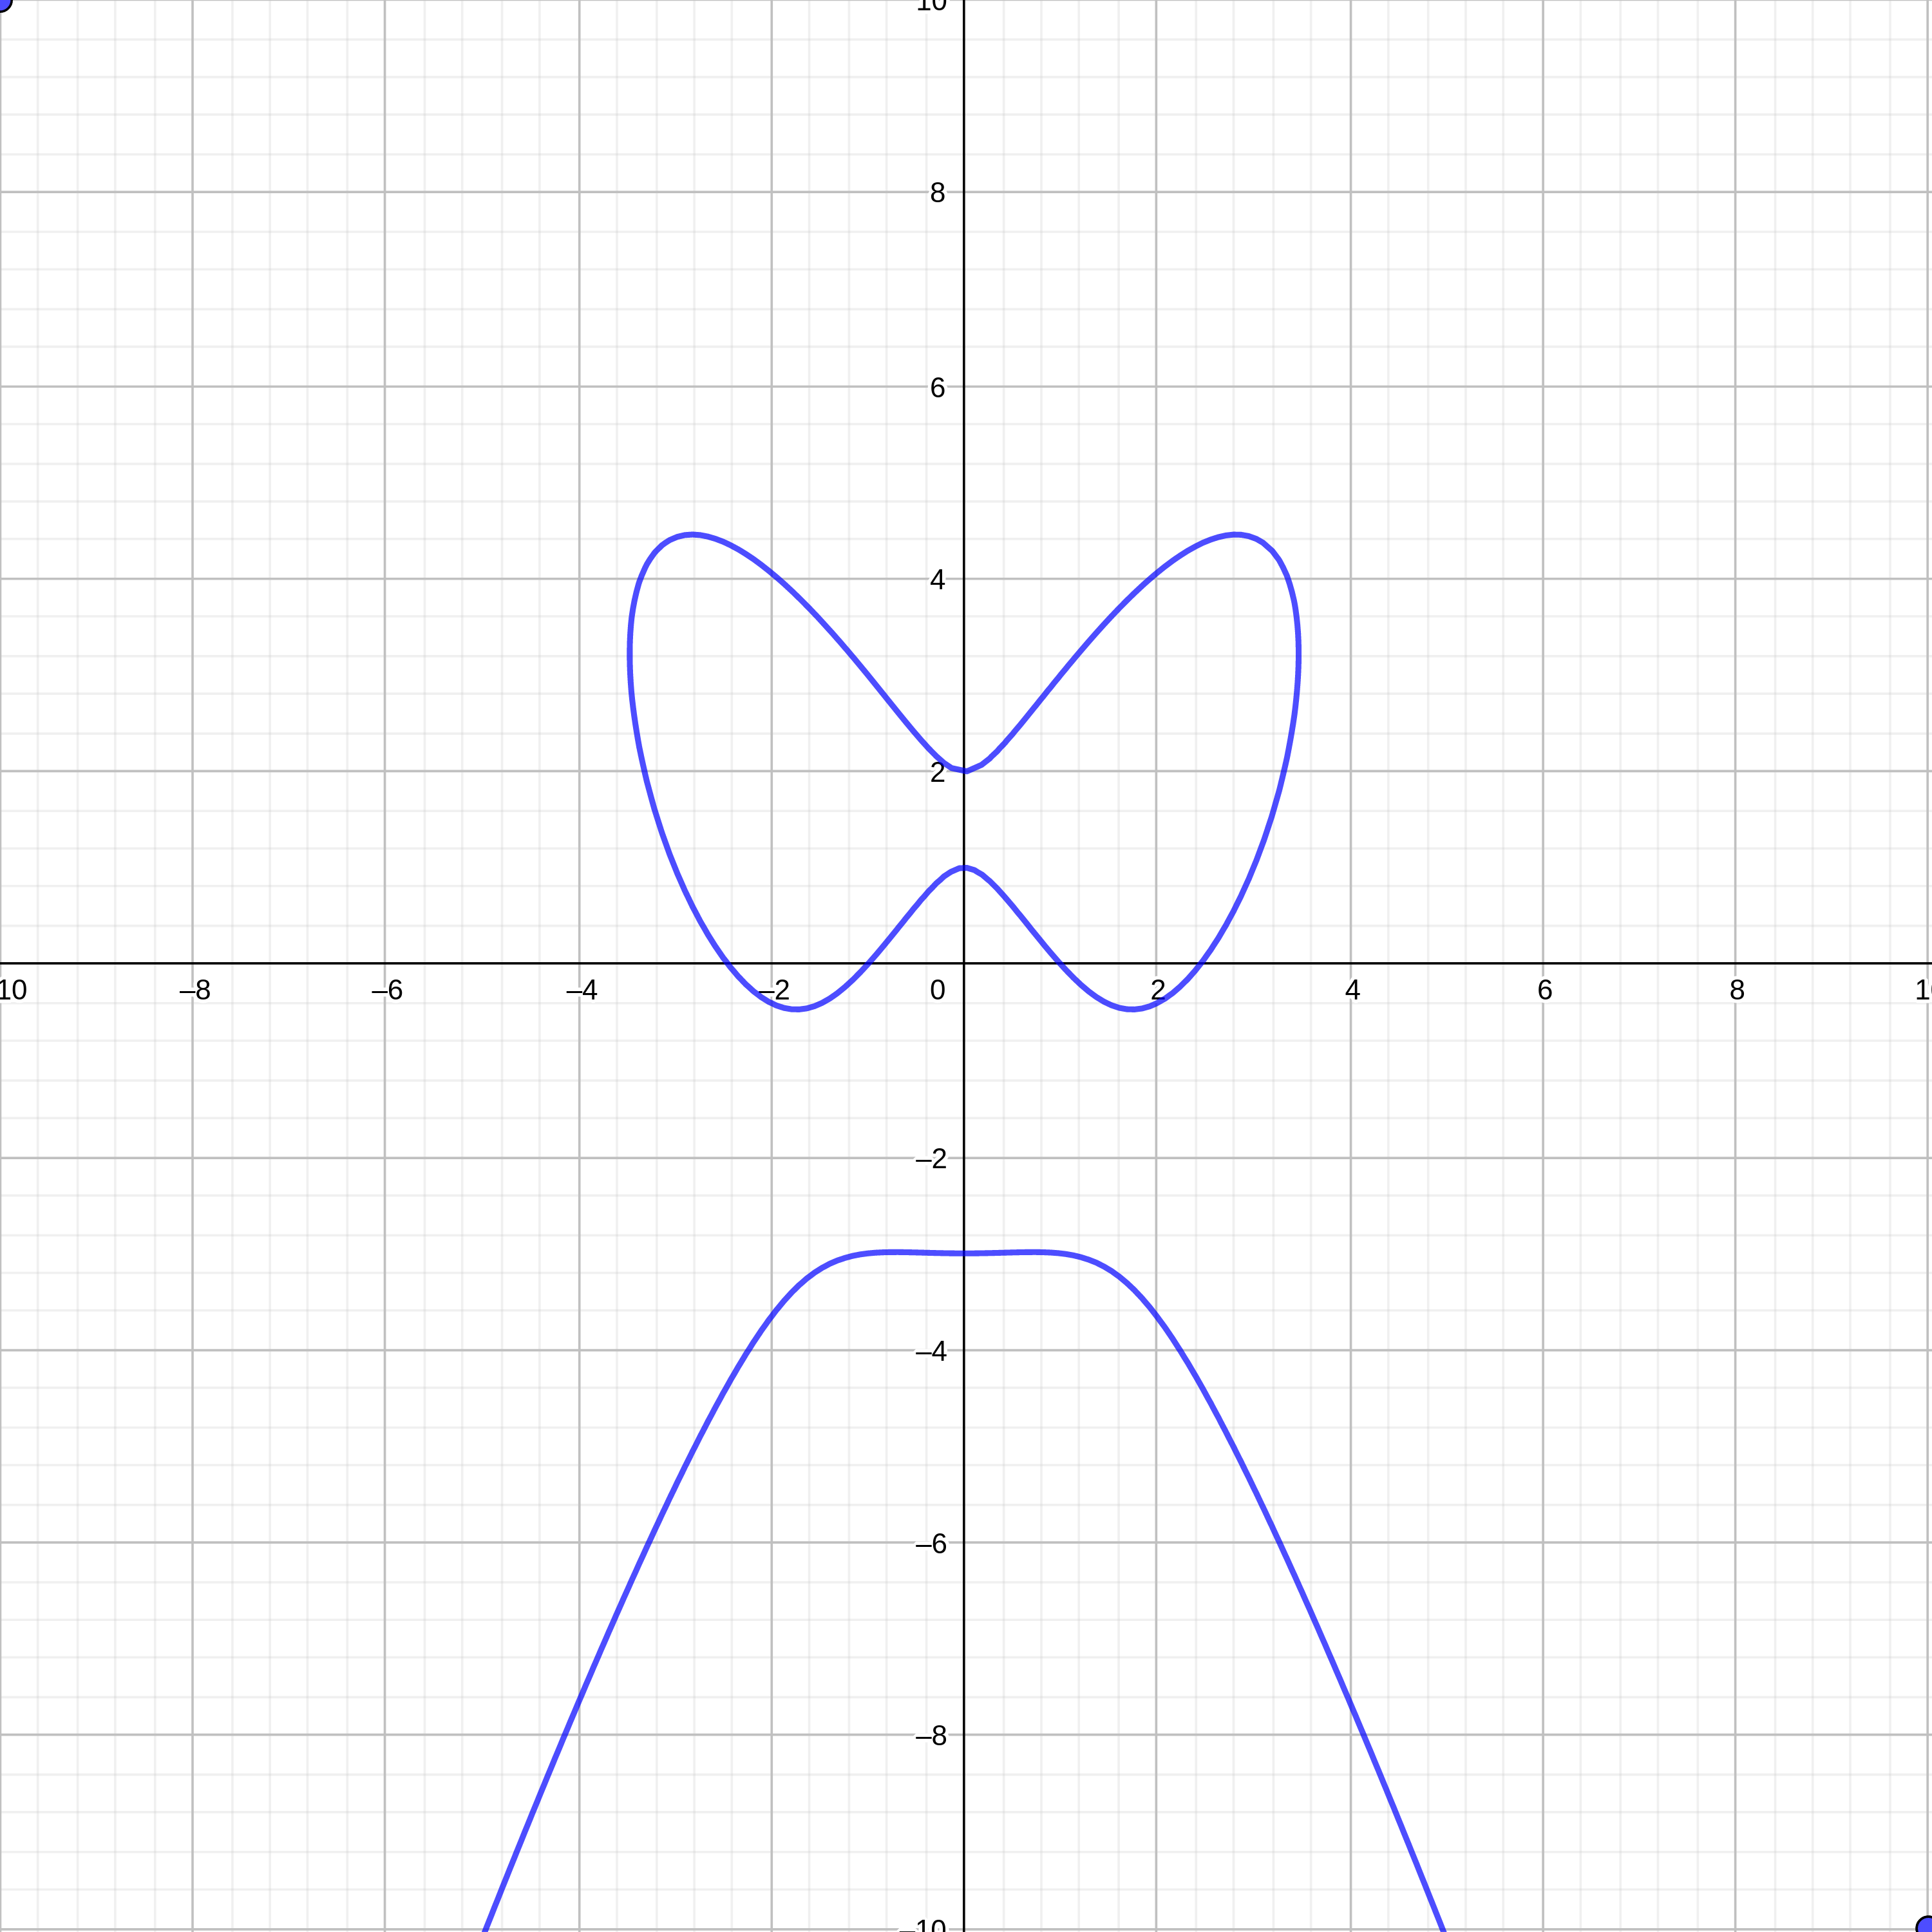
\includegraphics[height=7.6cm]{curve1.png} \end{center}
\end{frame}
\begin{frame}
\frametitle{Some $C_{3,4}$ Curves over $\bb R$}
  \begin{center} 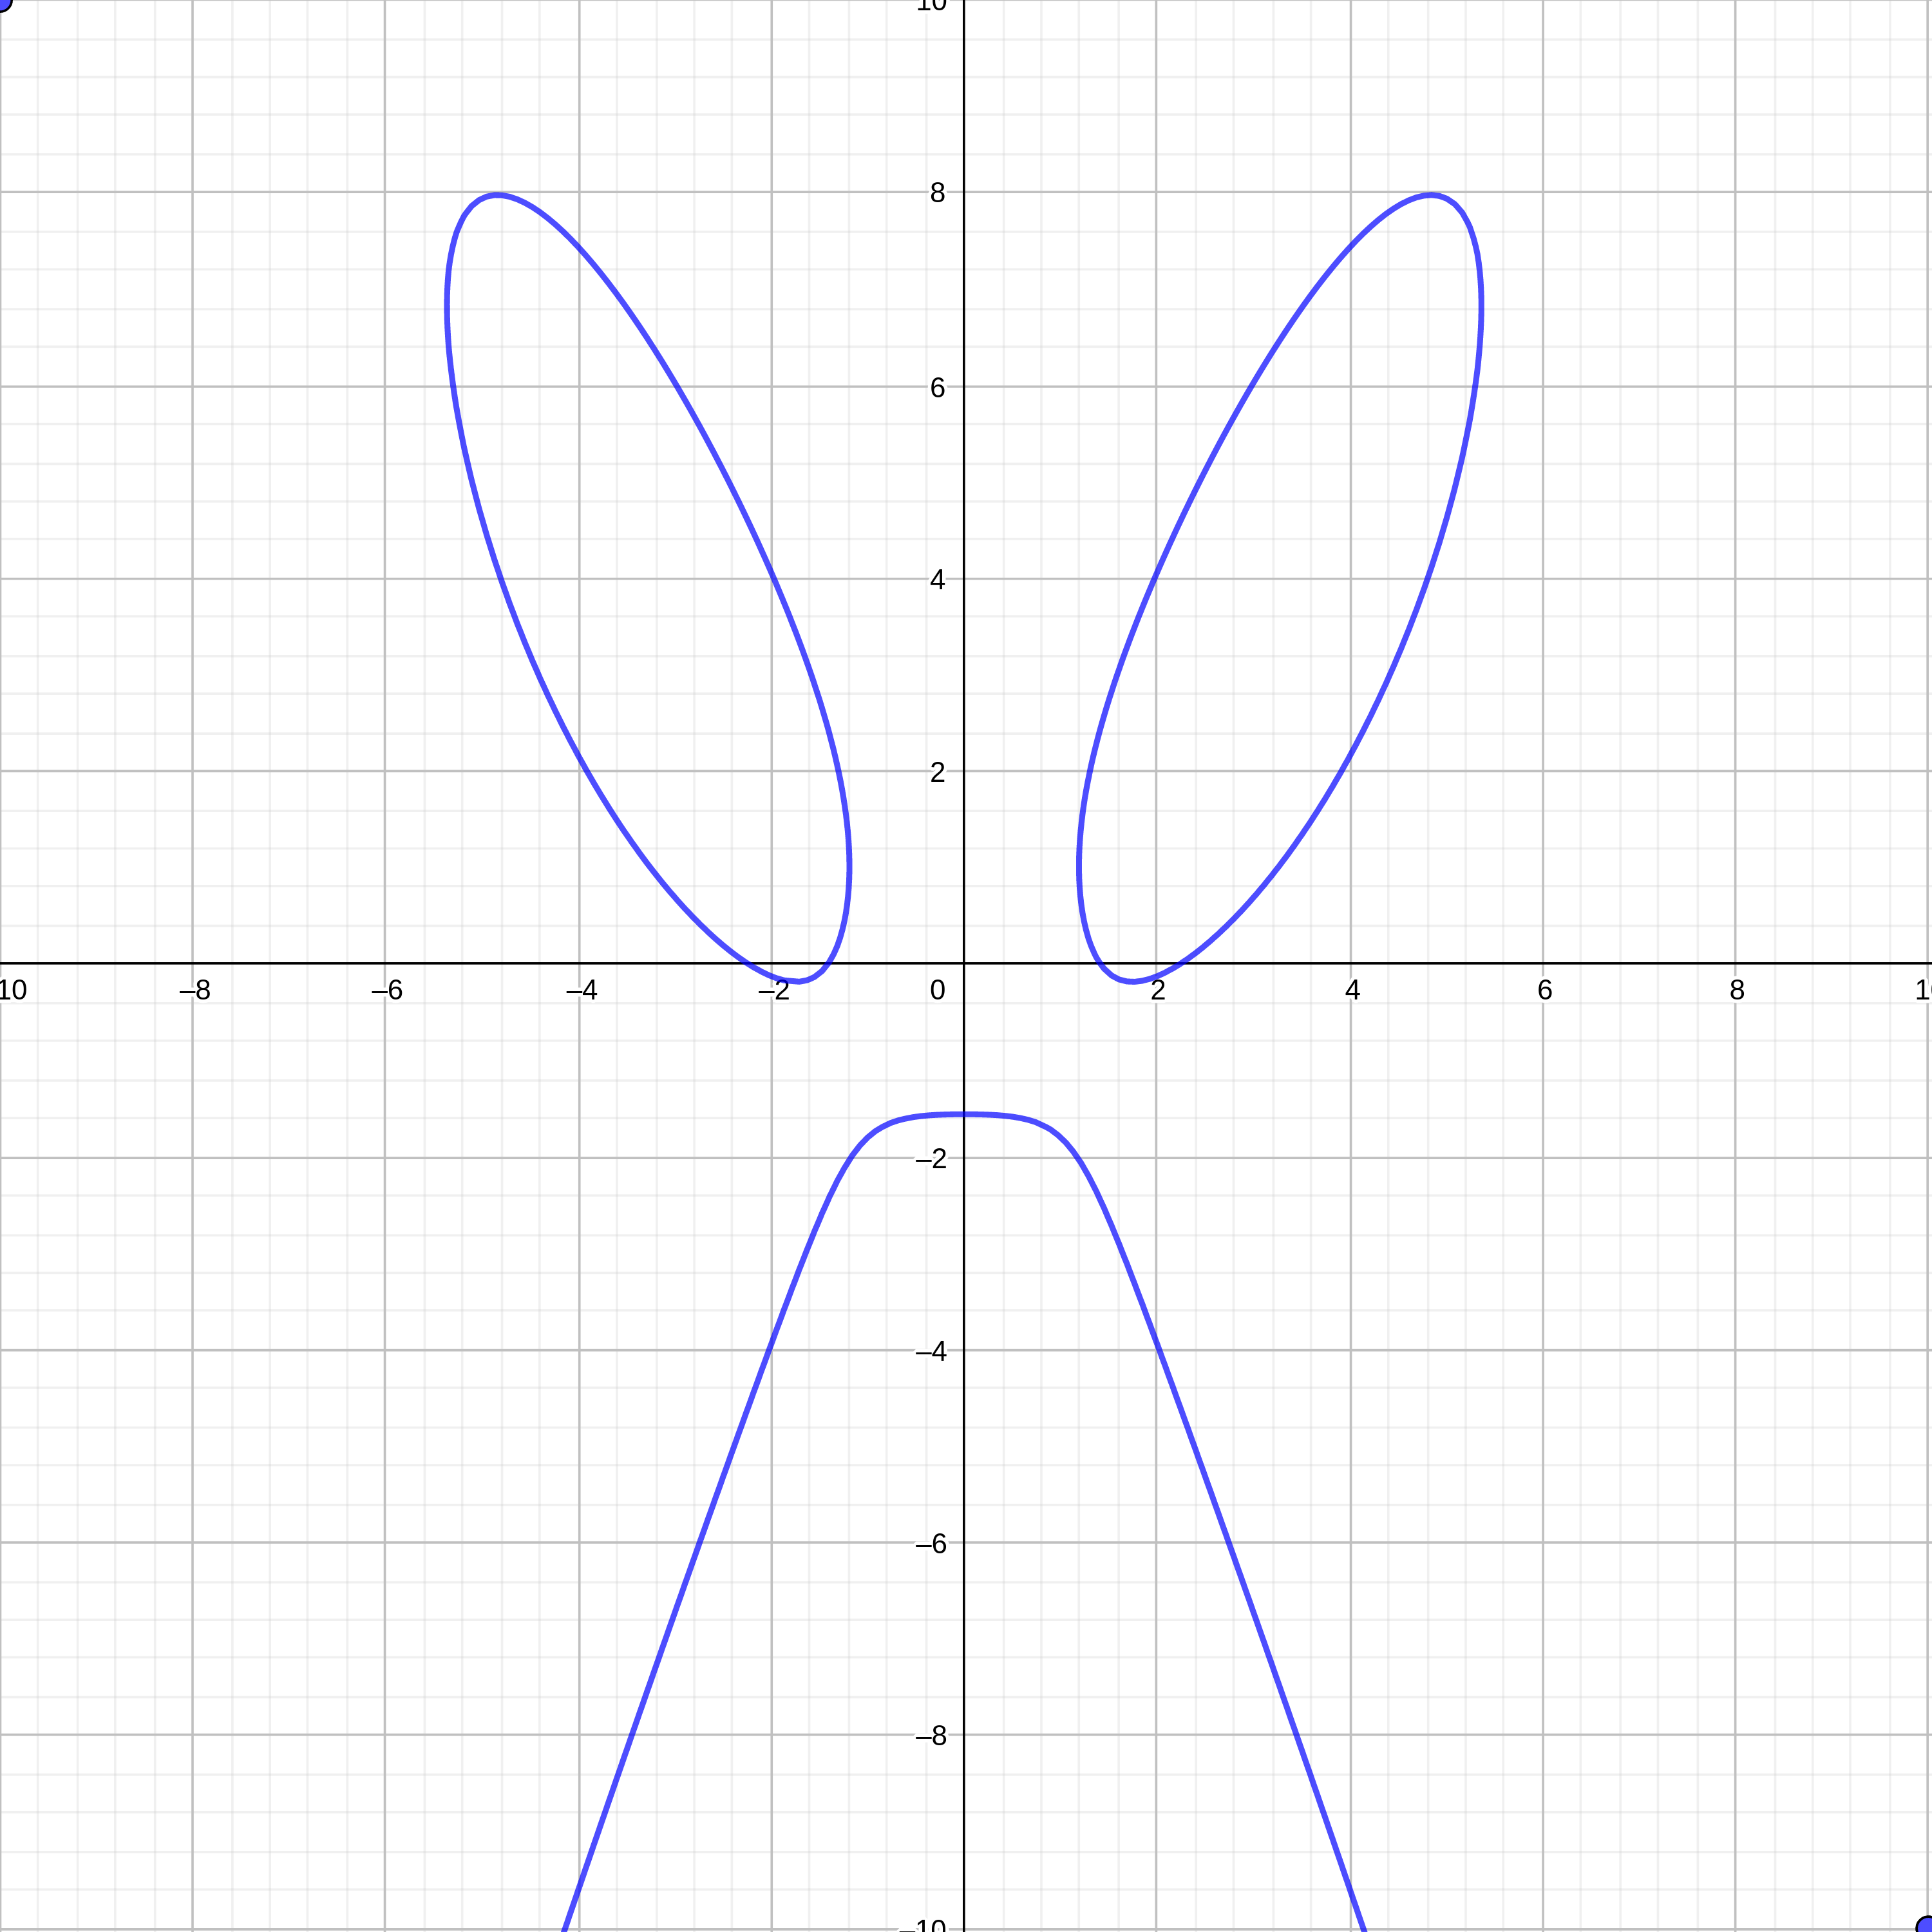
\includegraphics[height=7.6cm]{curve2.png} \end{center}
\end{frame}
\begin{frame}
\frametitle{Some $C_{3,4}$ Curves over $\bb R$}
  \begin{center} 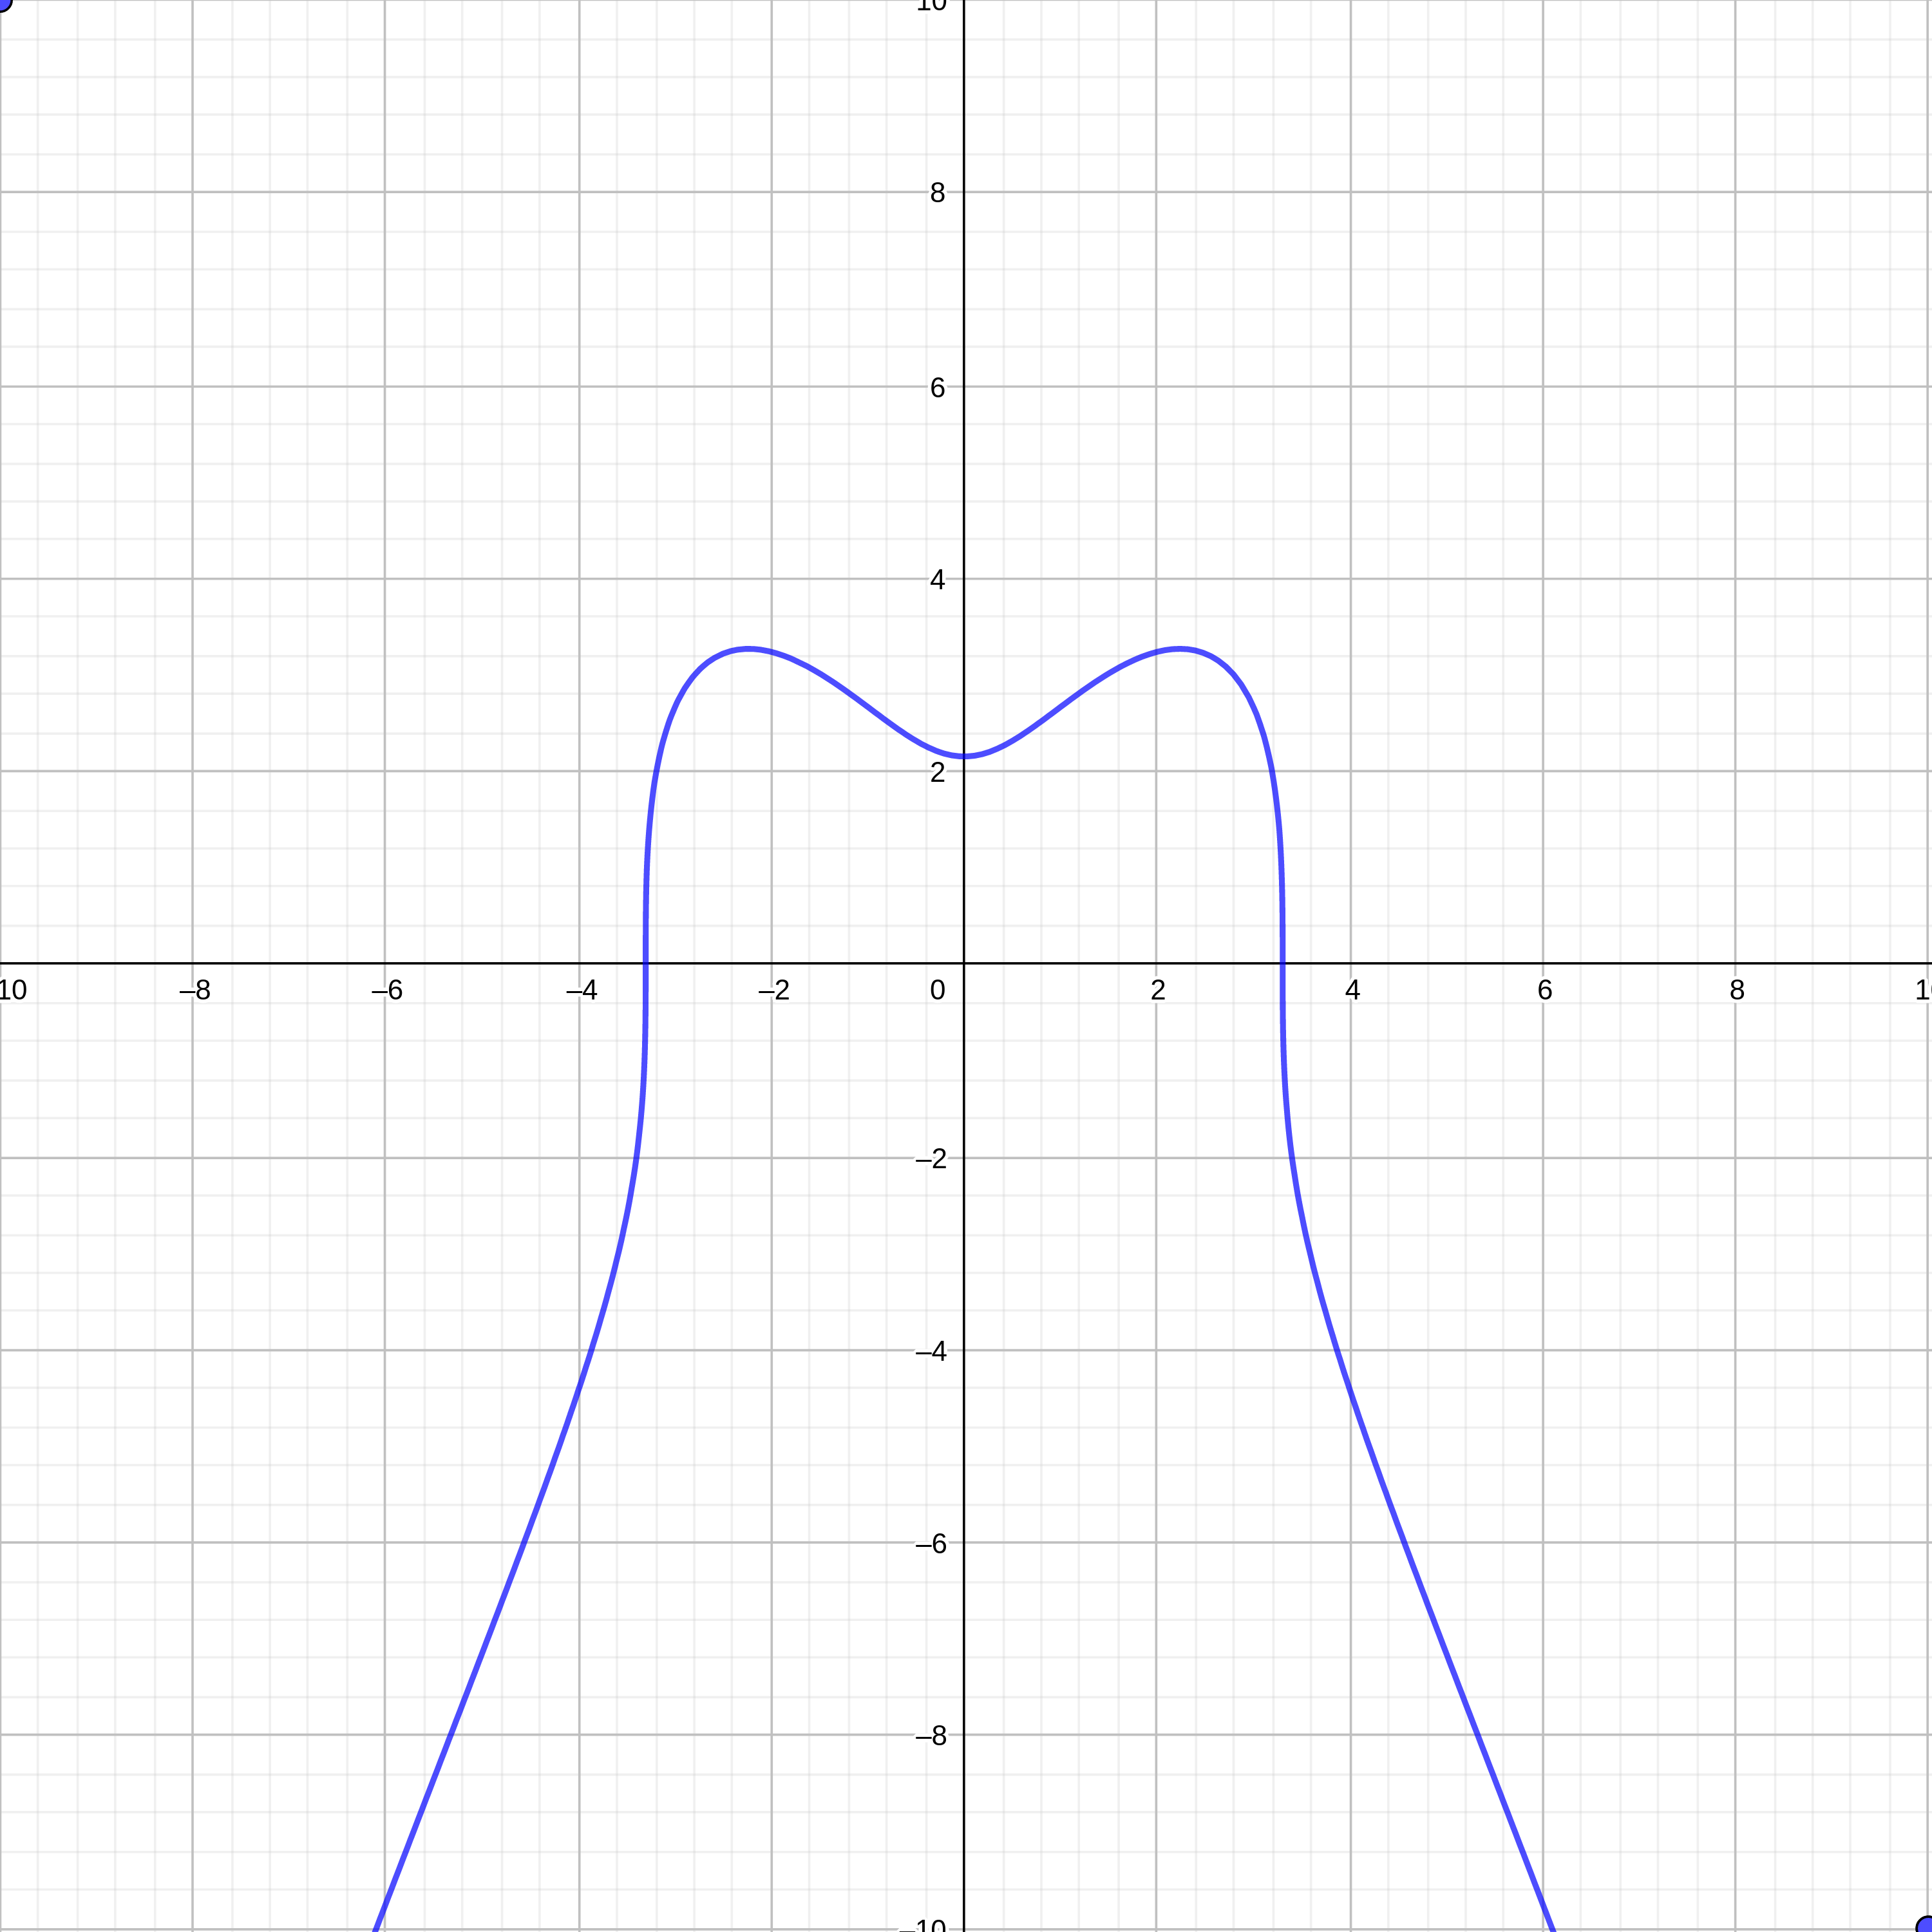
\includegraphics[height=7.6cm]{curve3.png} \end{center}
\end{frame}
\begin{frame}
\frametitle{Some $C_{3,4}$ Curves over $\bb R$}
  \begin{center} 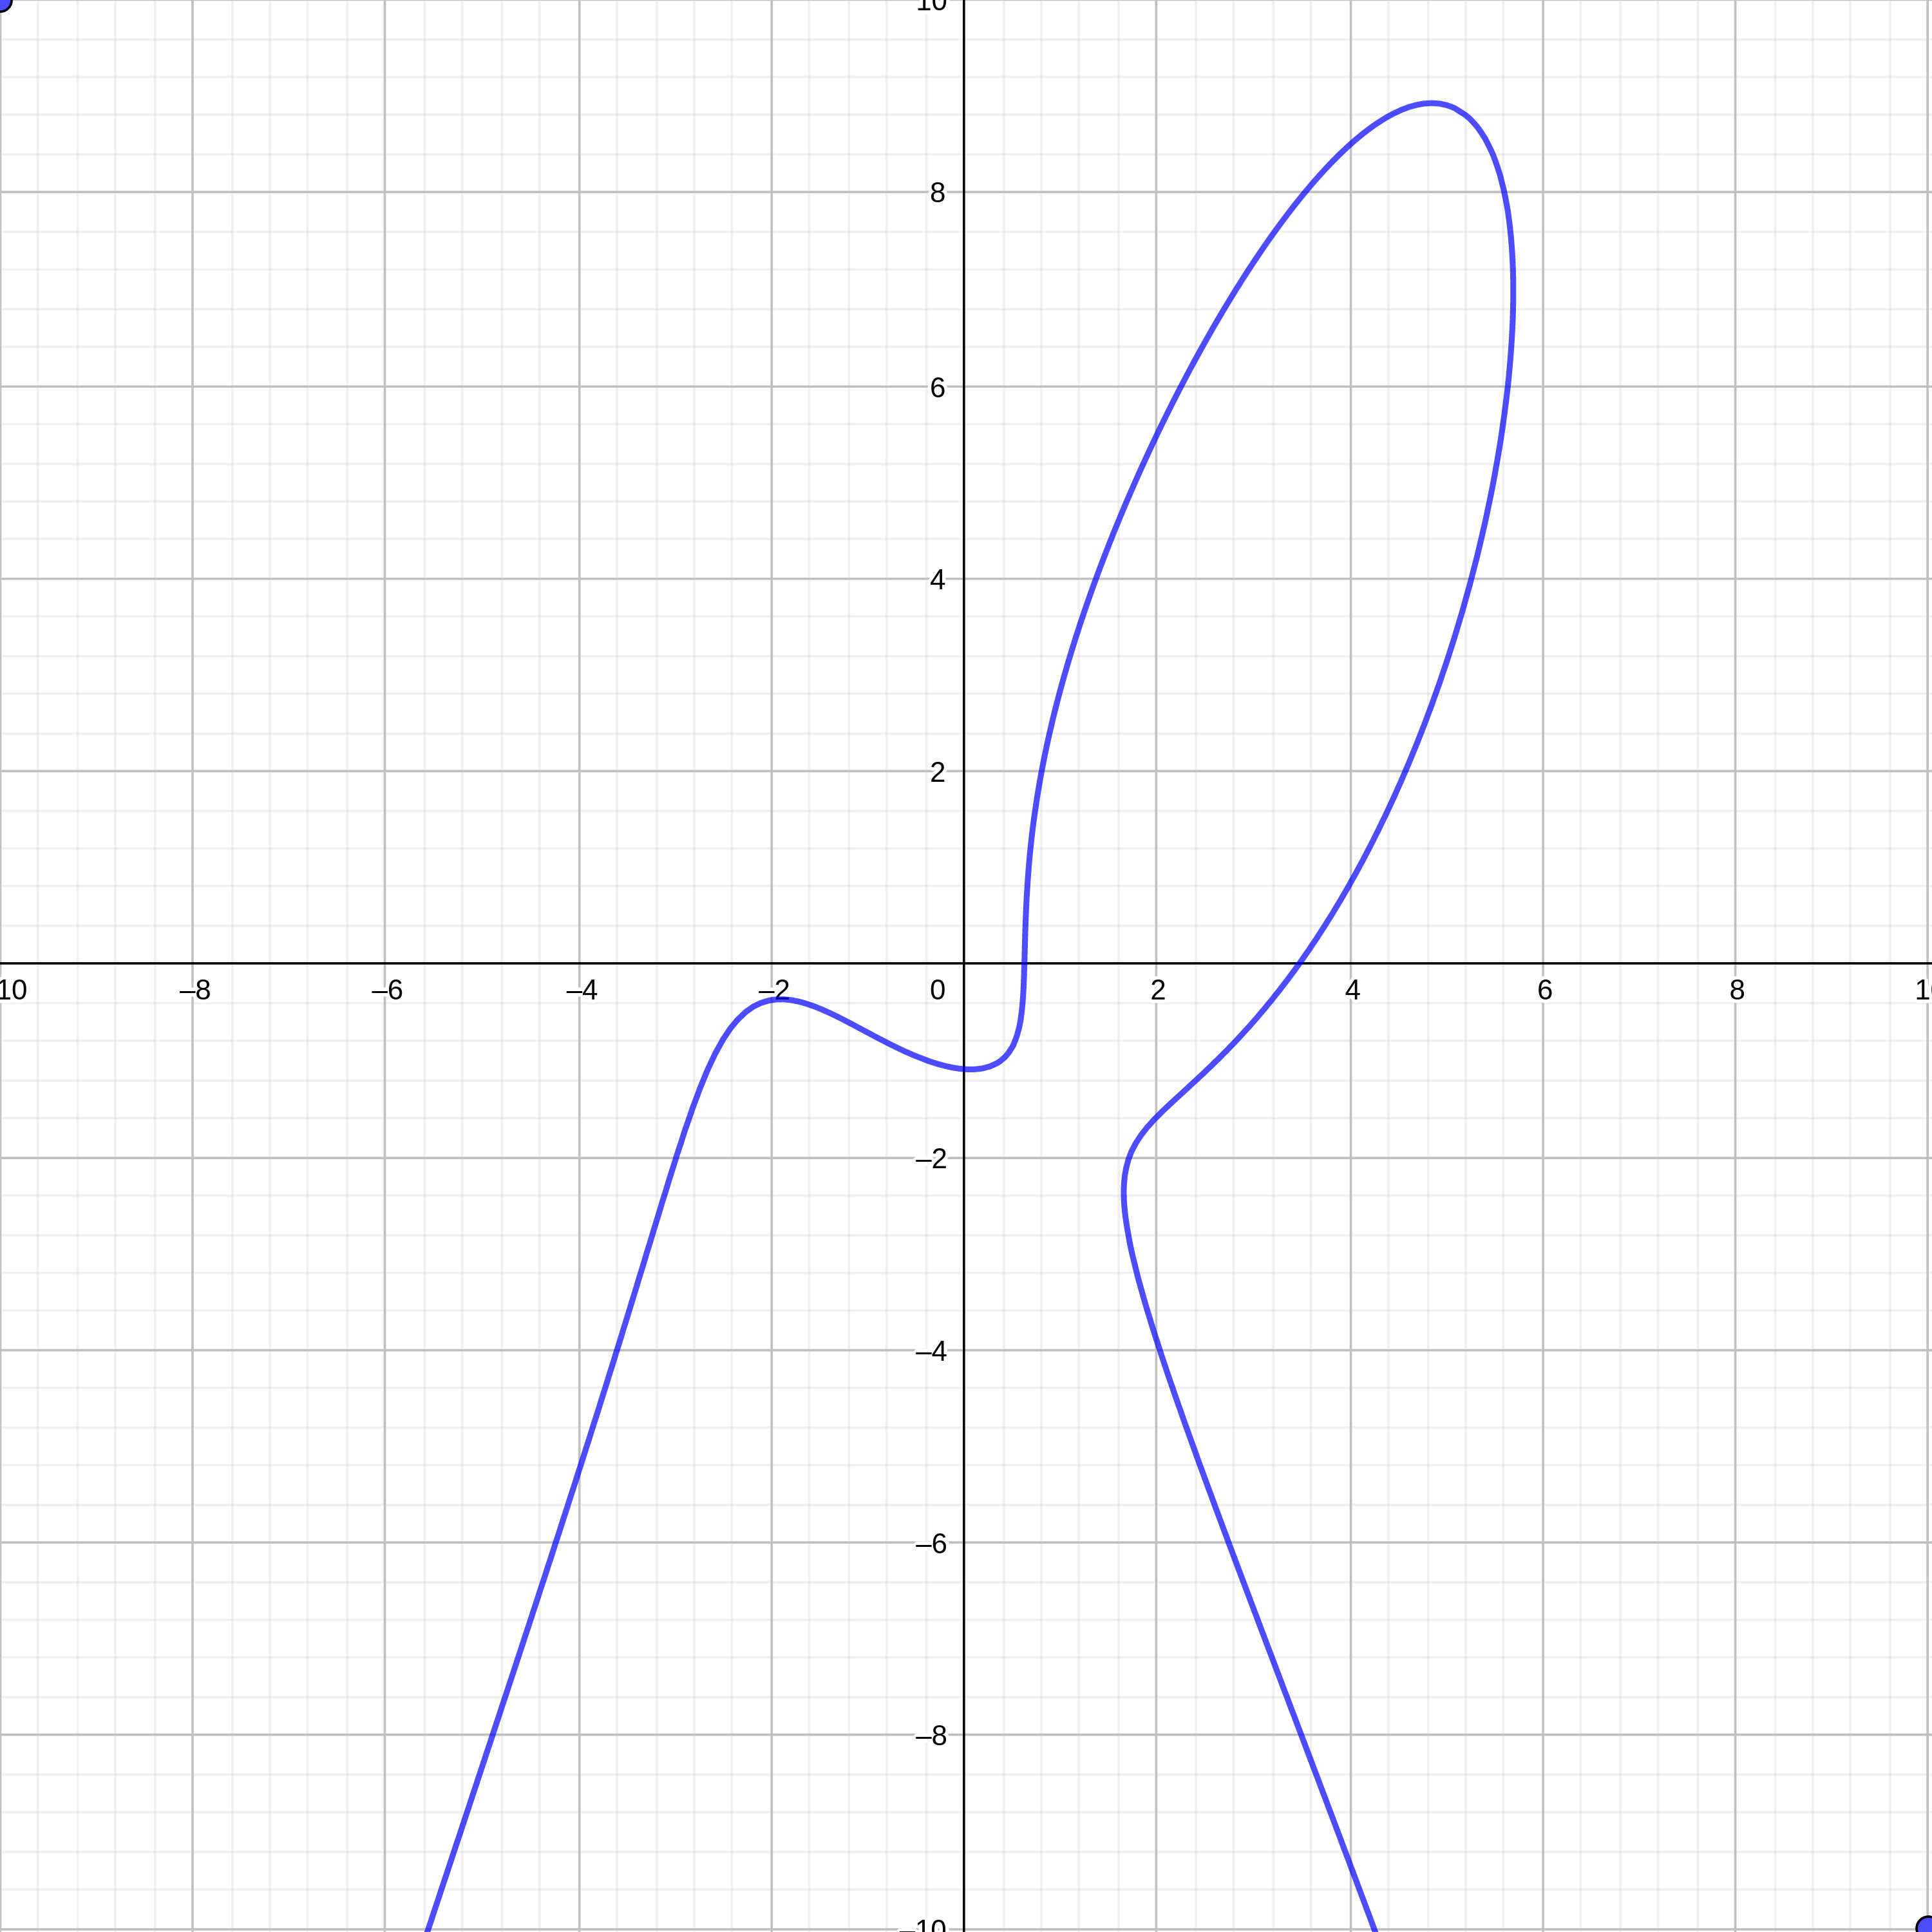
\includegraphics[height=7.6cm]{curve4.png} \end{center}
\end{frame}
%\end{comment}

%------------------------------------------------

\begin{frame}
\frametitle{What is a Divisor Class?}
  A \defn{divisor} of $C$ is a formal sum of points in $C(\bar K)$,
  \[ D = \sum_{P \in C(\bar K)} n_P P. \]
  Divisors form an Abelian group $\Div(C)$.\\
  \vspace{10pt}
  There is a chain of subgroups
  \[ \Princ(C) \subset \Div_K^0(C) \subset \Div^0(C) \subset \Div(C).\]
  The \defn{divisor class group} of $C$ is
  \[ \Cl(C) = \frac{\Div_K^0(C)}{\Princ(C)}.\]
\end{frame}

%------------------------------------------------

\begin{frame}
\frametitle{What is a Divisor Class?}
  The \defn{divisor of a rational function} $f$ is
  \[ \div f = \{ \text{zeros of $f$ on $C$} \} - \{ \text{poles of $f$ on $C$} \}.\]
  If $D = \div f$ for some $f$, $D$ is called \defn{principal}.\\
  Principal divisors lead to an equivalence relation
  \[ D \equiv D' \iff D - D' = \div f \text{ for some $f \in K(x,y)/F$}.\]
  Every divisor is equivalent to one of the form
  \[ D = P_1 + \dots + P_n - nP_\infty \]
  and can be represented by an ideal
  \[ I_D = \{ f \in K[x,y]/F ~:~ f(P_i) = 0 \}. \]
\end{frame}

%------------------------------------------------

\begin{frame}
\frametitle{The Goal}
  \begin{center}
    A divisor class $[D]$ has a unique ``reduced'' representative,
    \[ D = P_1 + \ldots + P_n, ~~ n \leq 3. \]
  \end{center}
  \vspace{10pt}
  \begin{center}
    Given two reduced divisors,\\
    find explicit formulas describing their reduced sum.
  \end{center}
\end{frame}

%------------------------------------------------

\begin{frame}
\frametitle{Why?}
  \begin{itemize}
    \item Part of an ongoing project at UofC to fully describe divisor arithmetic on genus 3 curves
    \item Testing generalizations of elliptic curve conjectures to genus 3
    \begin{itemize}
      \item Sato-Tate Conjecture
      \item Birch and Swinnerton-Dyer Conjecture
      \item and more ...
    \end{itemize}
    \item $L$-series computations
  \end{itemize}
\end{frame}

%------------------------------------------------

\begin{frame}
\frametitle{Previous Work}
  Arita (2005) \footcite{arita05-2}
  \begin{itemize}
    \item $\Char K > 3$
    \item Inputs: any two reduced divisors
    \item Non-disjoint case: handled randomly, recursively, might not terminate on some silly curves
    \item Slow, computes redundant or unnecessary values
    \item Classification of divisors of degree $\leq 6$ into 20 types
  \end{itemize}
\end{frame}

%------------------------------------------------

\begin{frame}
  Flon et al. (2008, preprint in 2004)\footcite{flon08}
  \begin{itemize}
    \item $\Char K > 3$
    \item Inputs and outputs must be ``typical'' and reduced
    \item Non-disjoint case: unhandled
  \end{itemize}
  \vspace{10pt}
  Khuri-Makdisi and Abu Salem (2007)\footcite{kamal07}
  \begin{itemize}
    \item Same setting as above, but faster
  \end{itemize}
  \vspace{10pt}
  Khuri-Makdisi (2018)\footcite{kamal18}
  \begin{itemize}
    \item Improvement over 2007
    \item Current state-of-the-art for typical case
  \end{itemize}
\end{frame}

%------------------------------------------------

\begin{frame}
\frametitle{Operations}
  \[ \text{Divisor class group of $C$} \simeq \text{Ideal class group of $K[x,y]/F$}\]
  \[ D \longleftrightarrow I_D \]
  Represent a divisor $D$ by the unique reduced Gr\"obner basis (RGB) of $I_D$. \\
  %A \defn{typical} reduced divisor has the form
  %\[ D \simeq I_D = \pid{\begin{array}{l}
  %  x^2 + f_2y + f_1x + f_0, \\
  %  xy + g_2y + g_1x + g_0, \\
  %  y^2 + h_2y + h_1x + h_0
  %  \end{array}} \]
  %with $f_2 \neq 0$.
  \begin{center}
    \begin{tabular}{c|c}
      Divisor & Ideal \\
      \hline
      $A + B$ & $I_A I_B$ \\
      $\lcm(A,B)$ & $I_A \cap I_B$ \\
      $\gcd(A,B)$ & $I_A + I_B$ \\
      $\bar A$ & $f : I_A$
    \end{tabular}
  \end{center}
  where $f$ is minimal in $I_A$.
\end{frame}

%------------------------------------------------

%\begin{comment}
\begin{frame}
\frametitle{$D$}
  \begin{center} 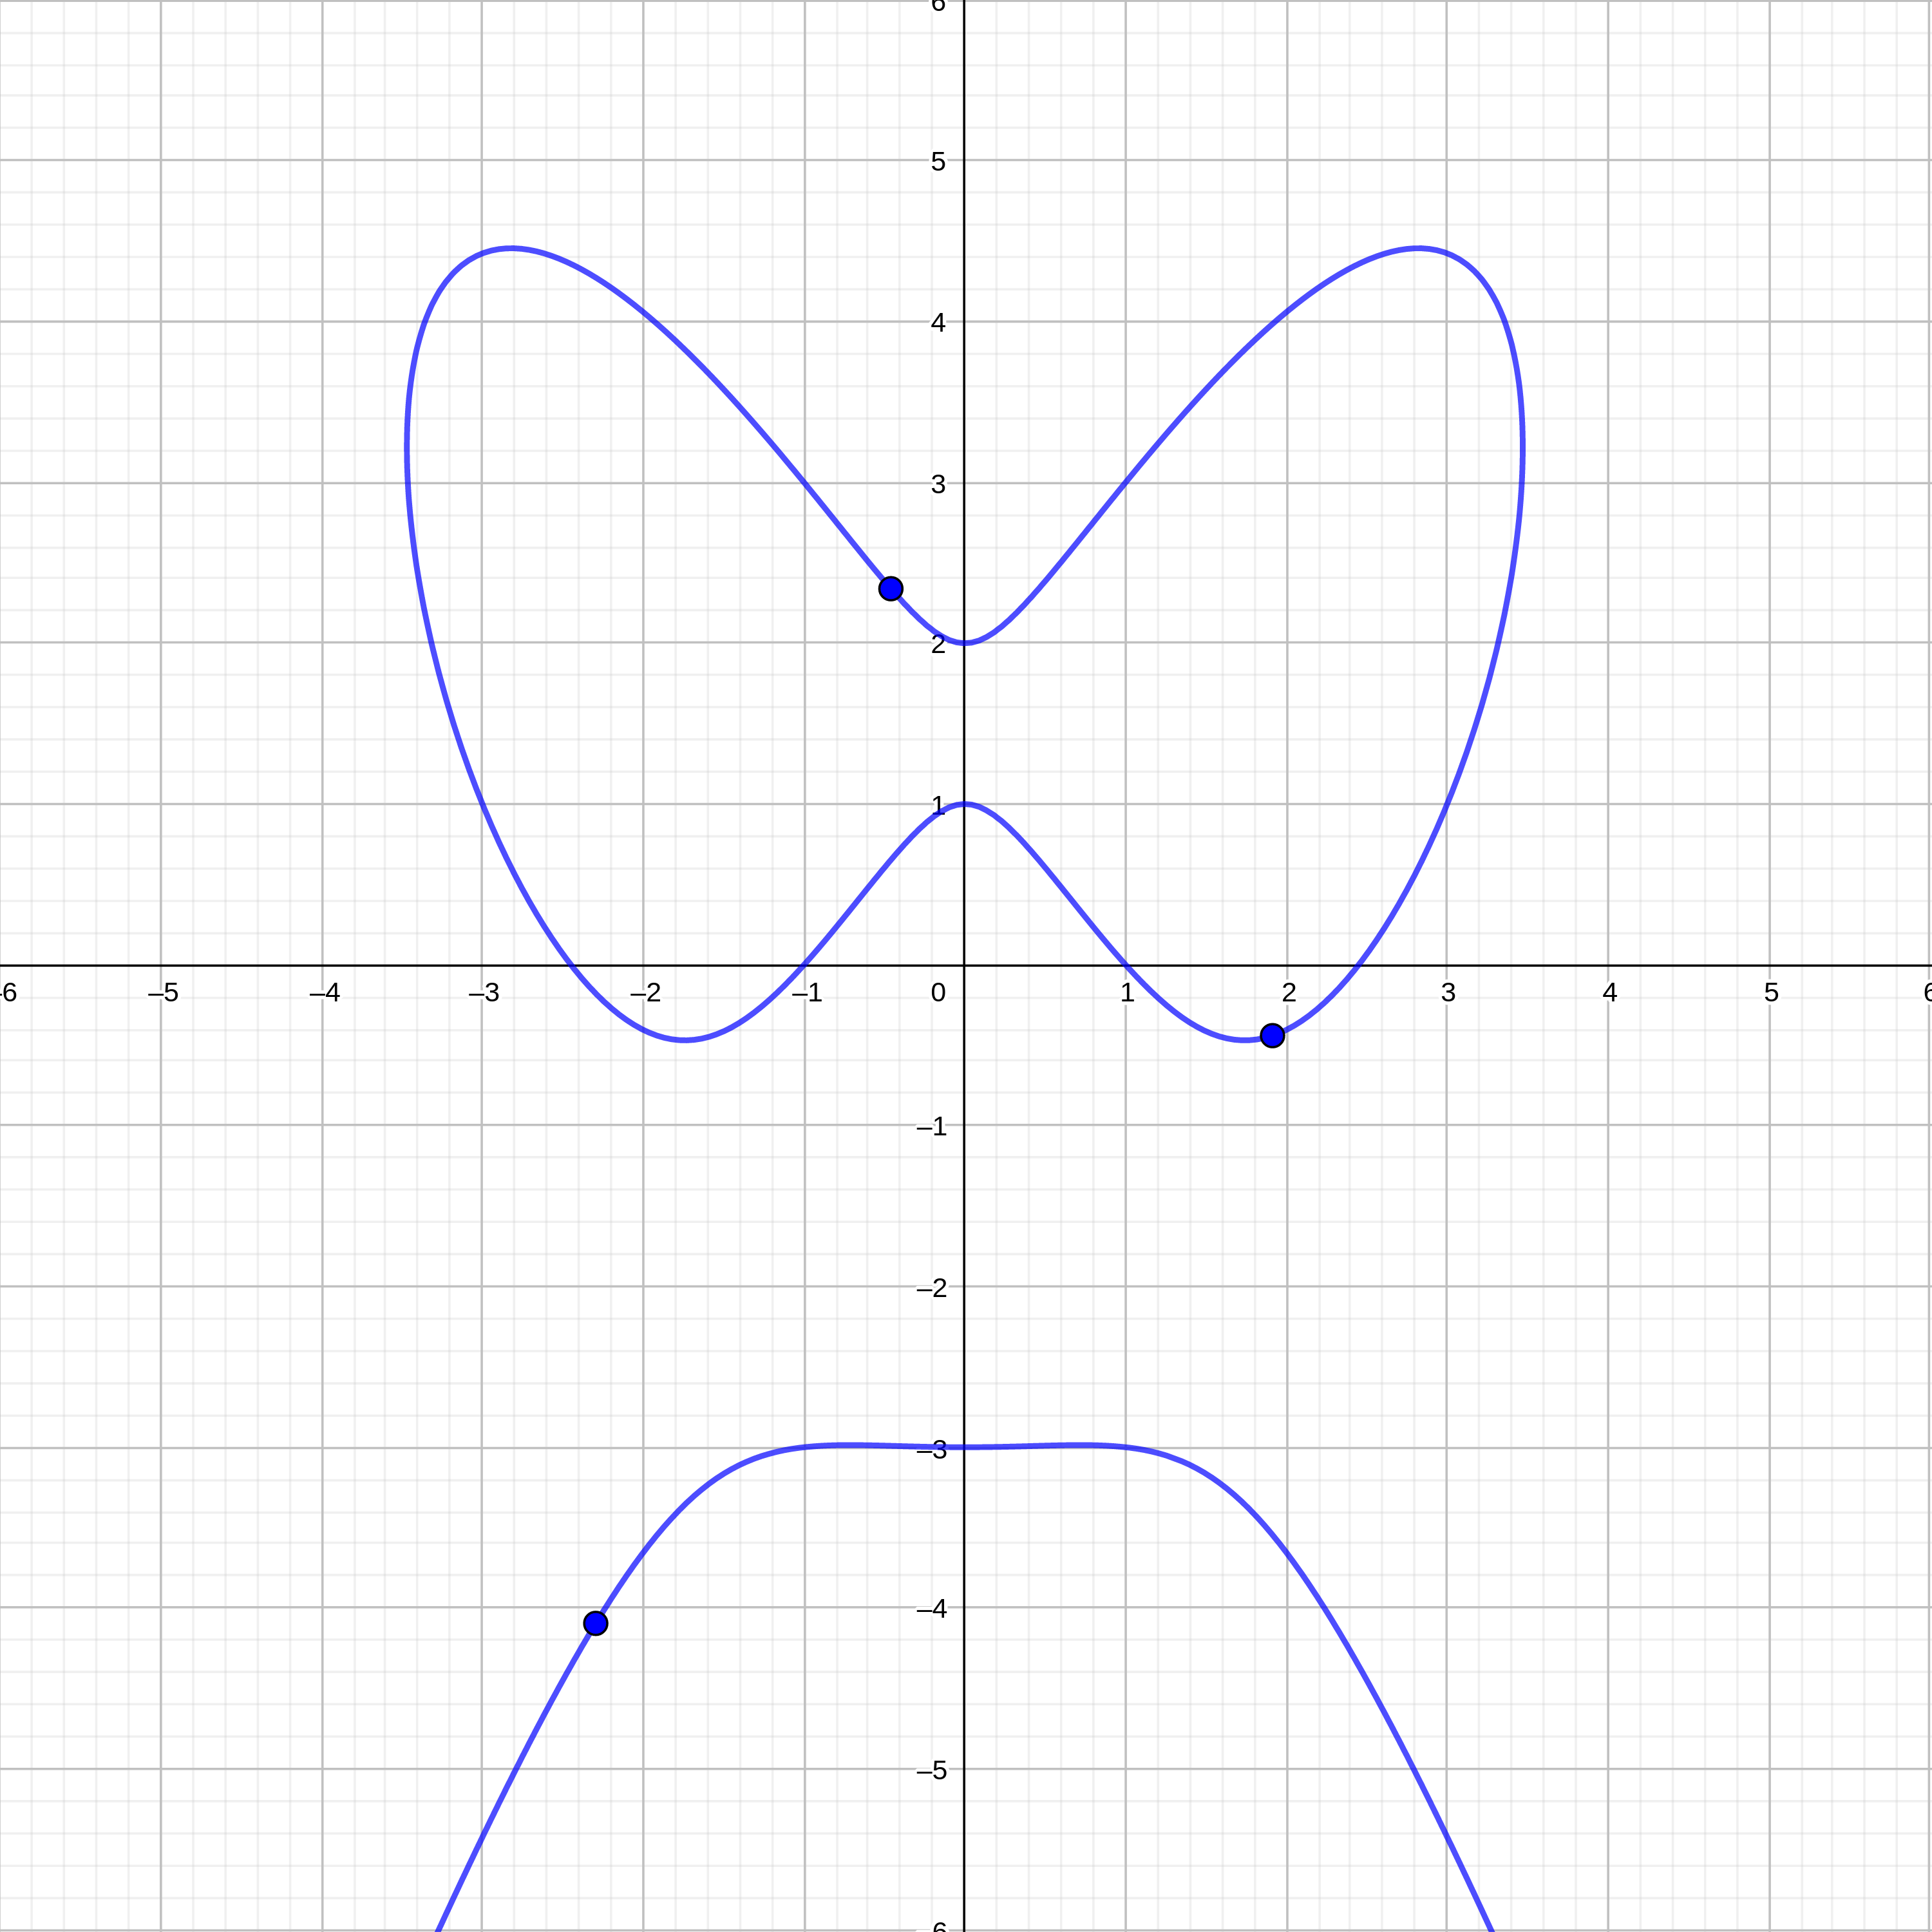
\includegraphics[height=7.6cm]{d1.png} \end{center}
\end{frame}
\begin{frame}
\frametitle{$D'$}
  \begin{center} 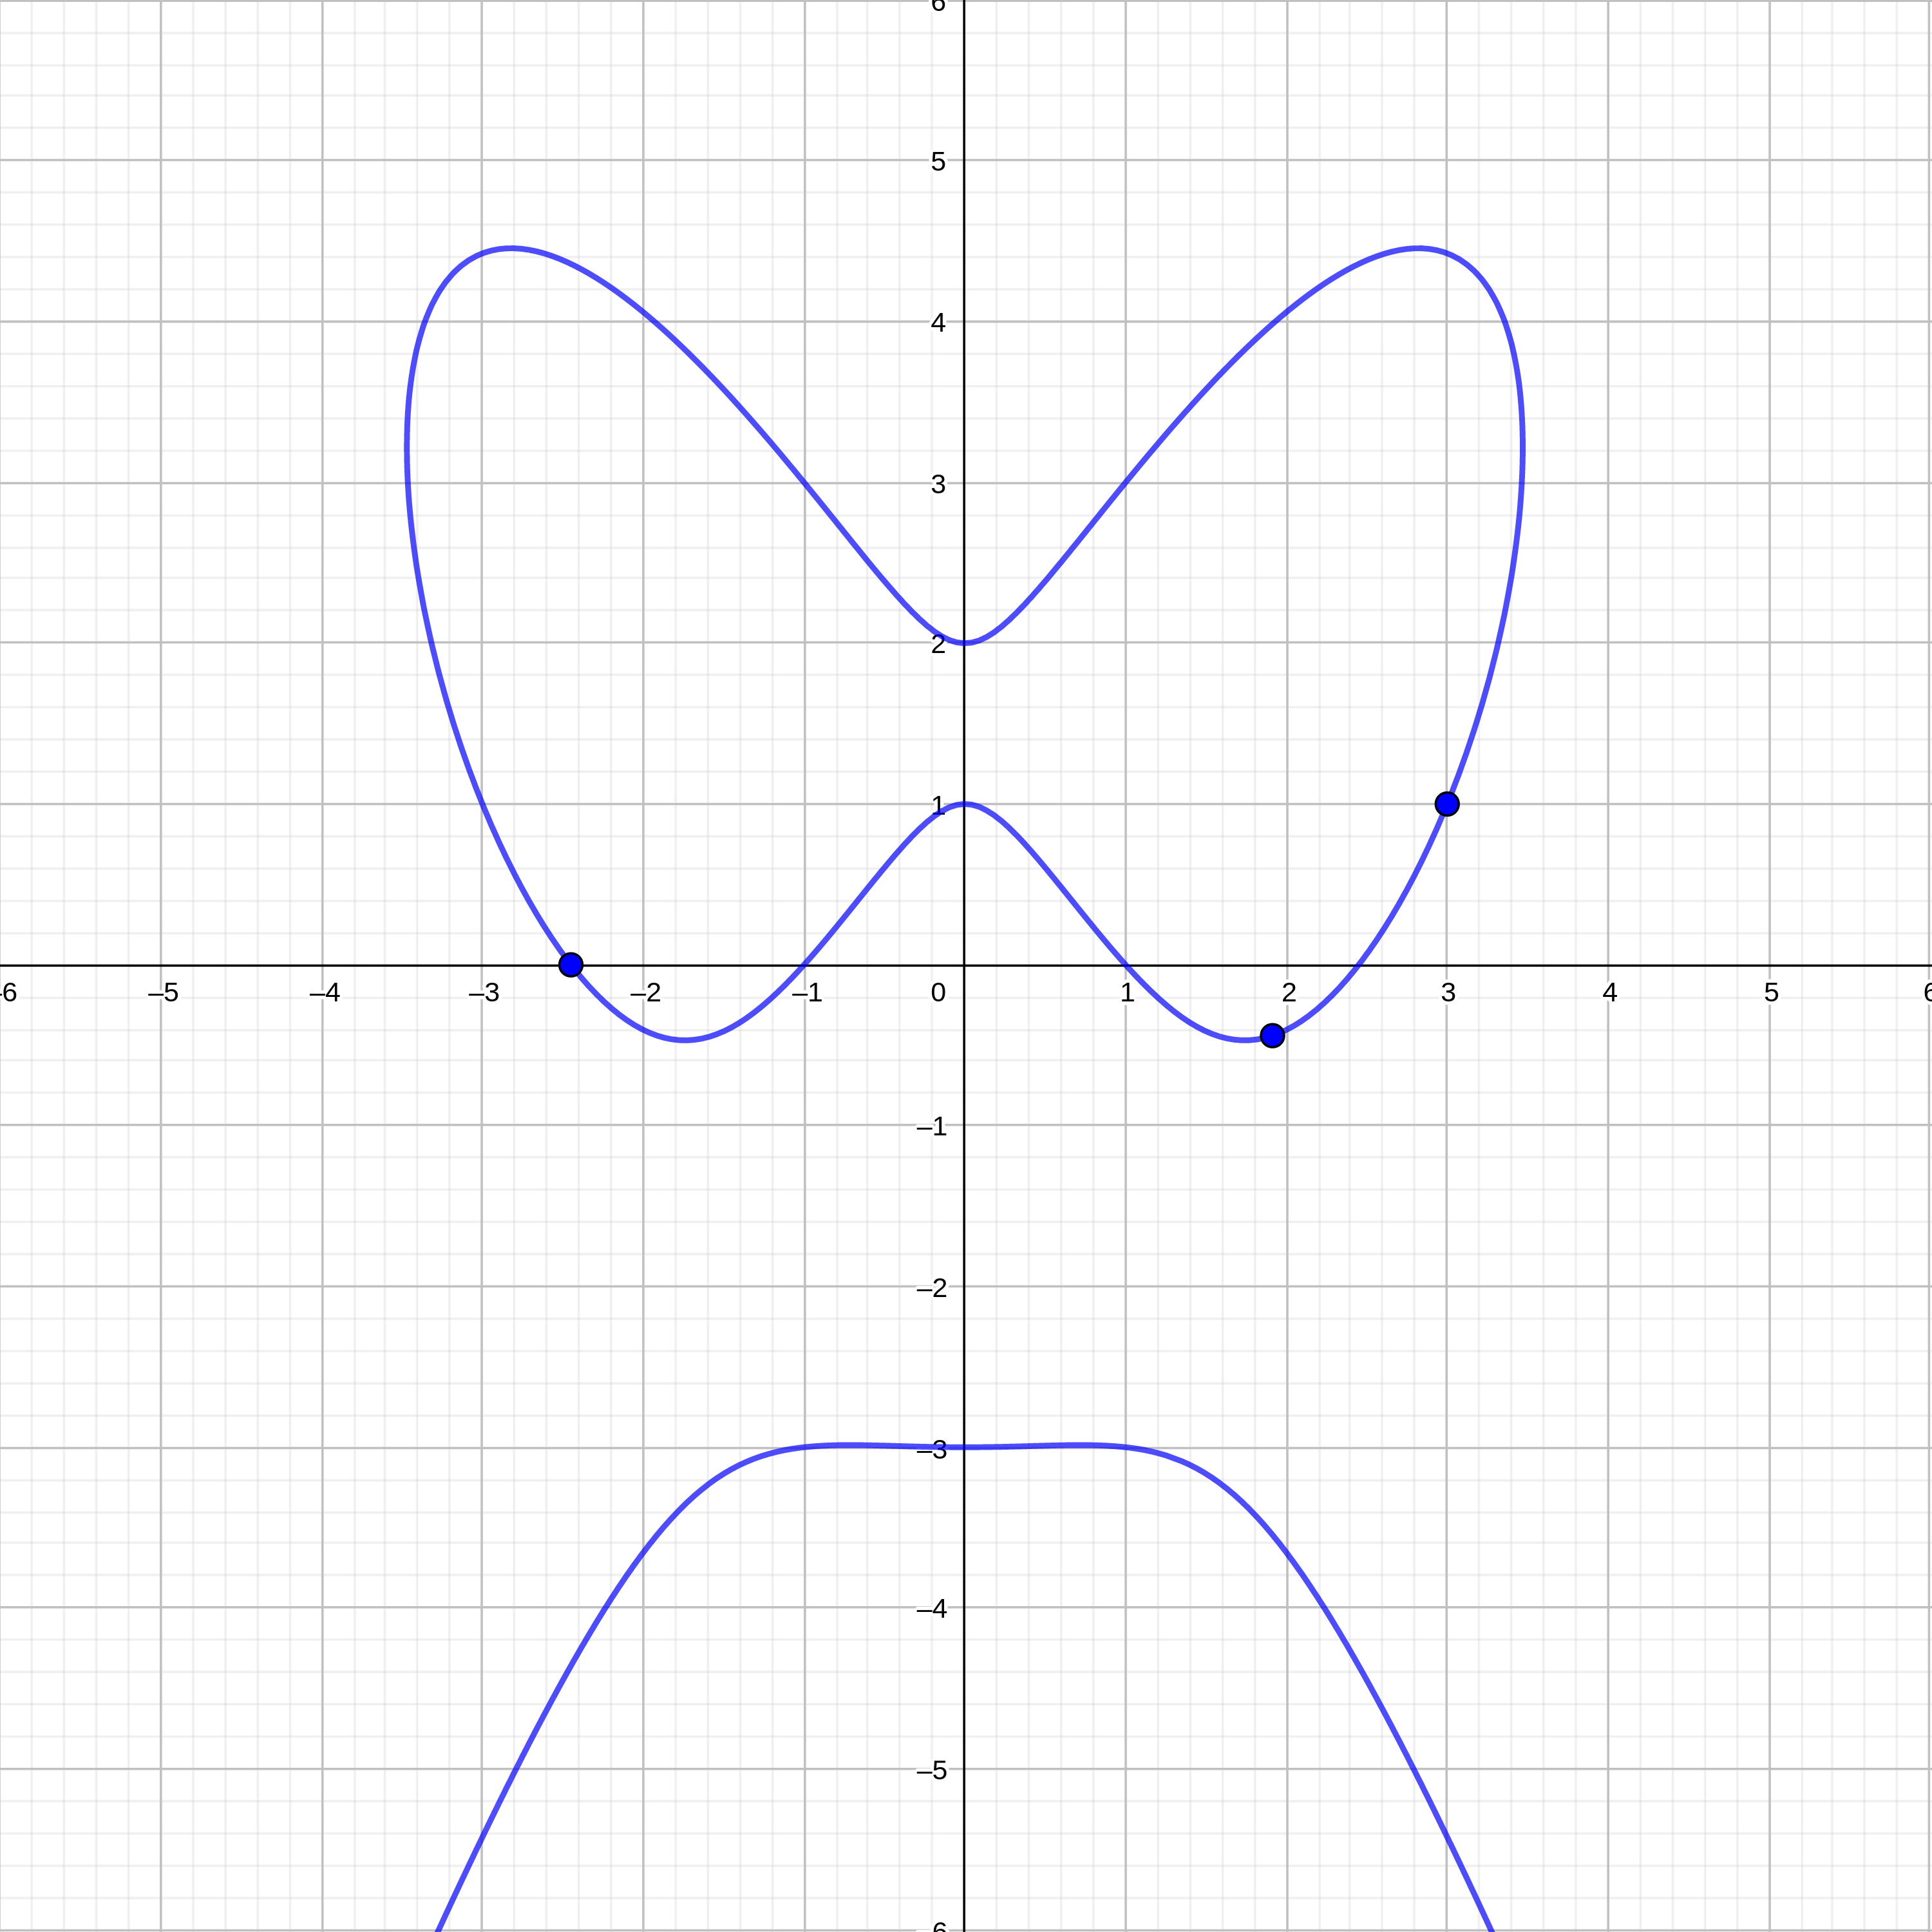
\includegraphics[height=7.6cm]{d2.png} \end{center}
\end{frame}
\begin{frame}
\frametitle{$D + D'$}
  \begin{center} 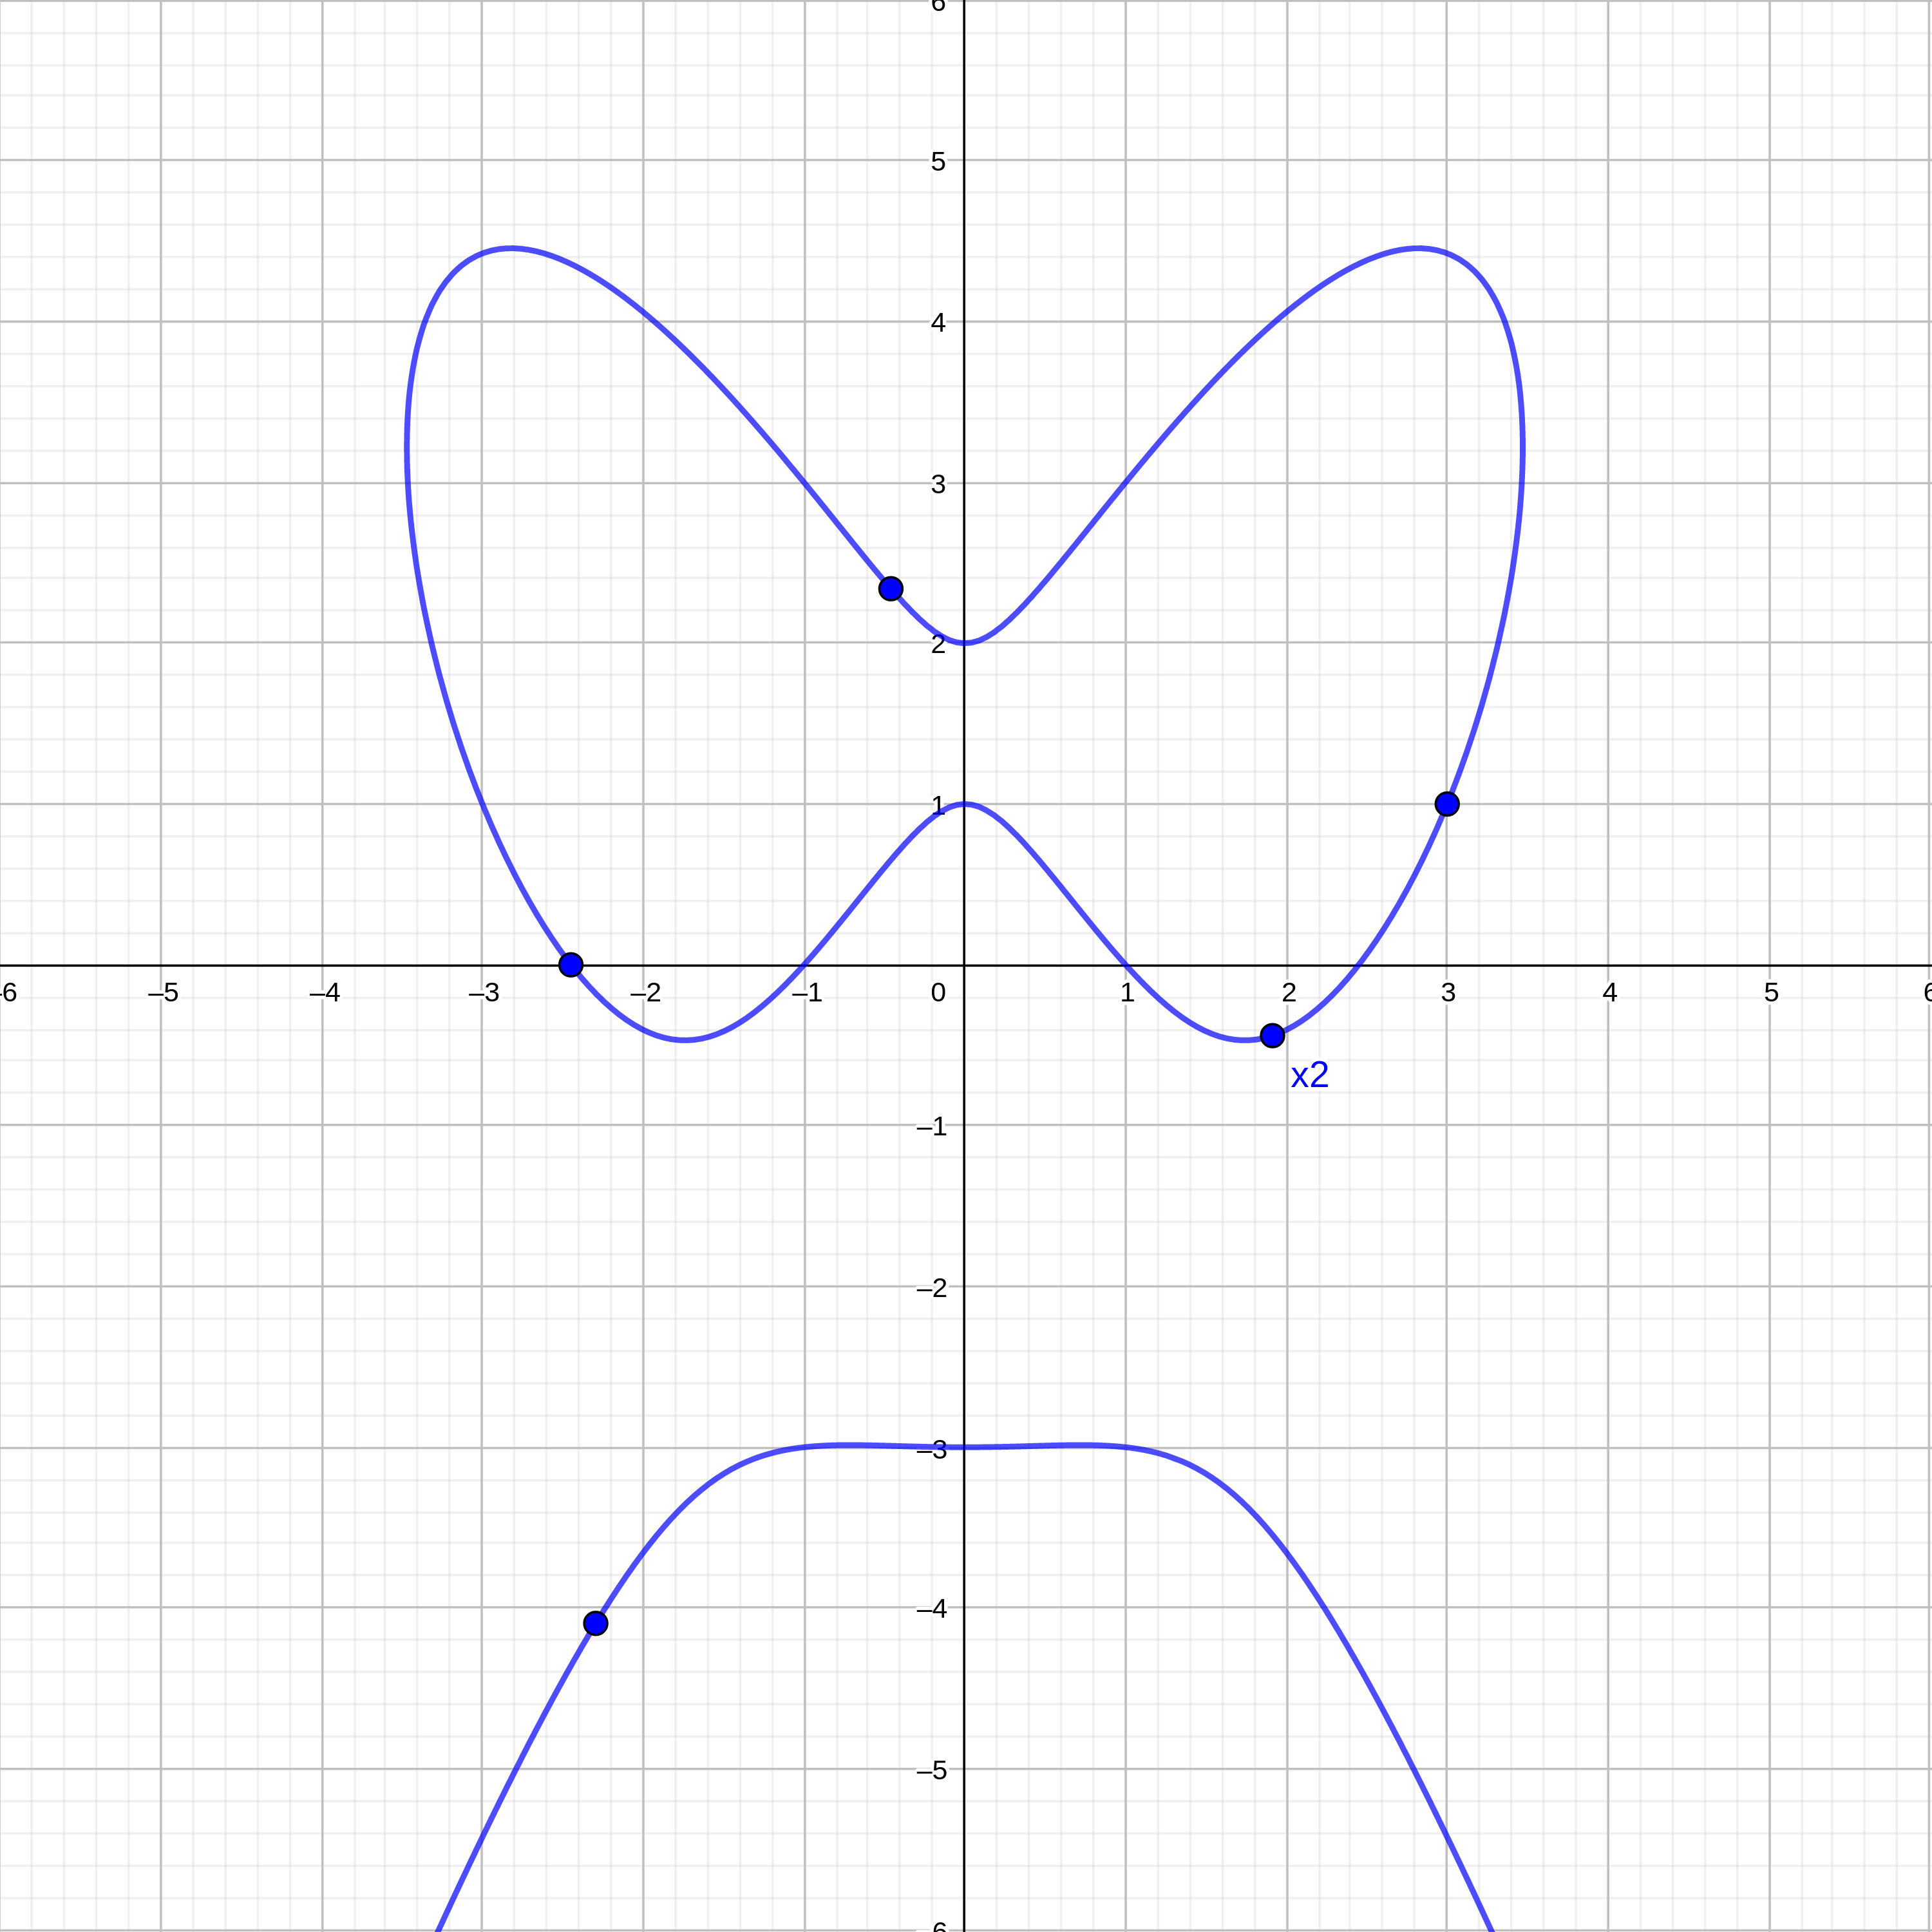
\includegraphics[height=7.6cm]{d1_d2.png} \end{center}
\end{frame}
\begin{frame}
\frametitle{$\lcm(D, D')$}
  \begin{center} 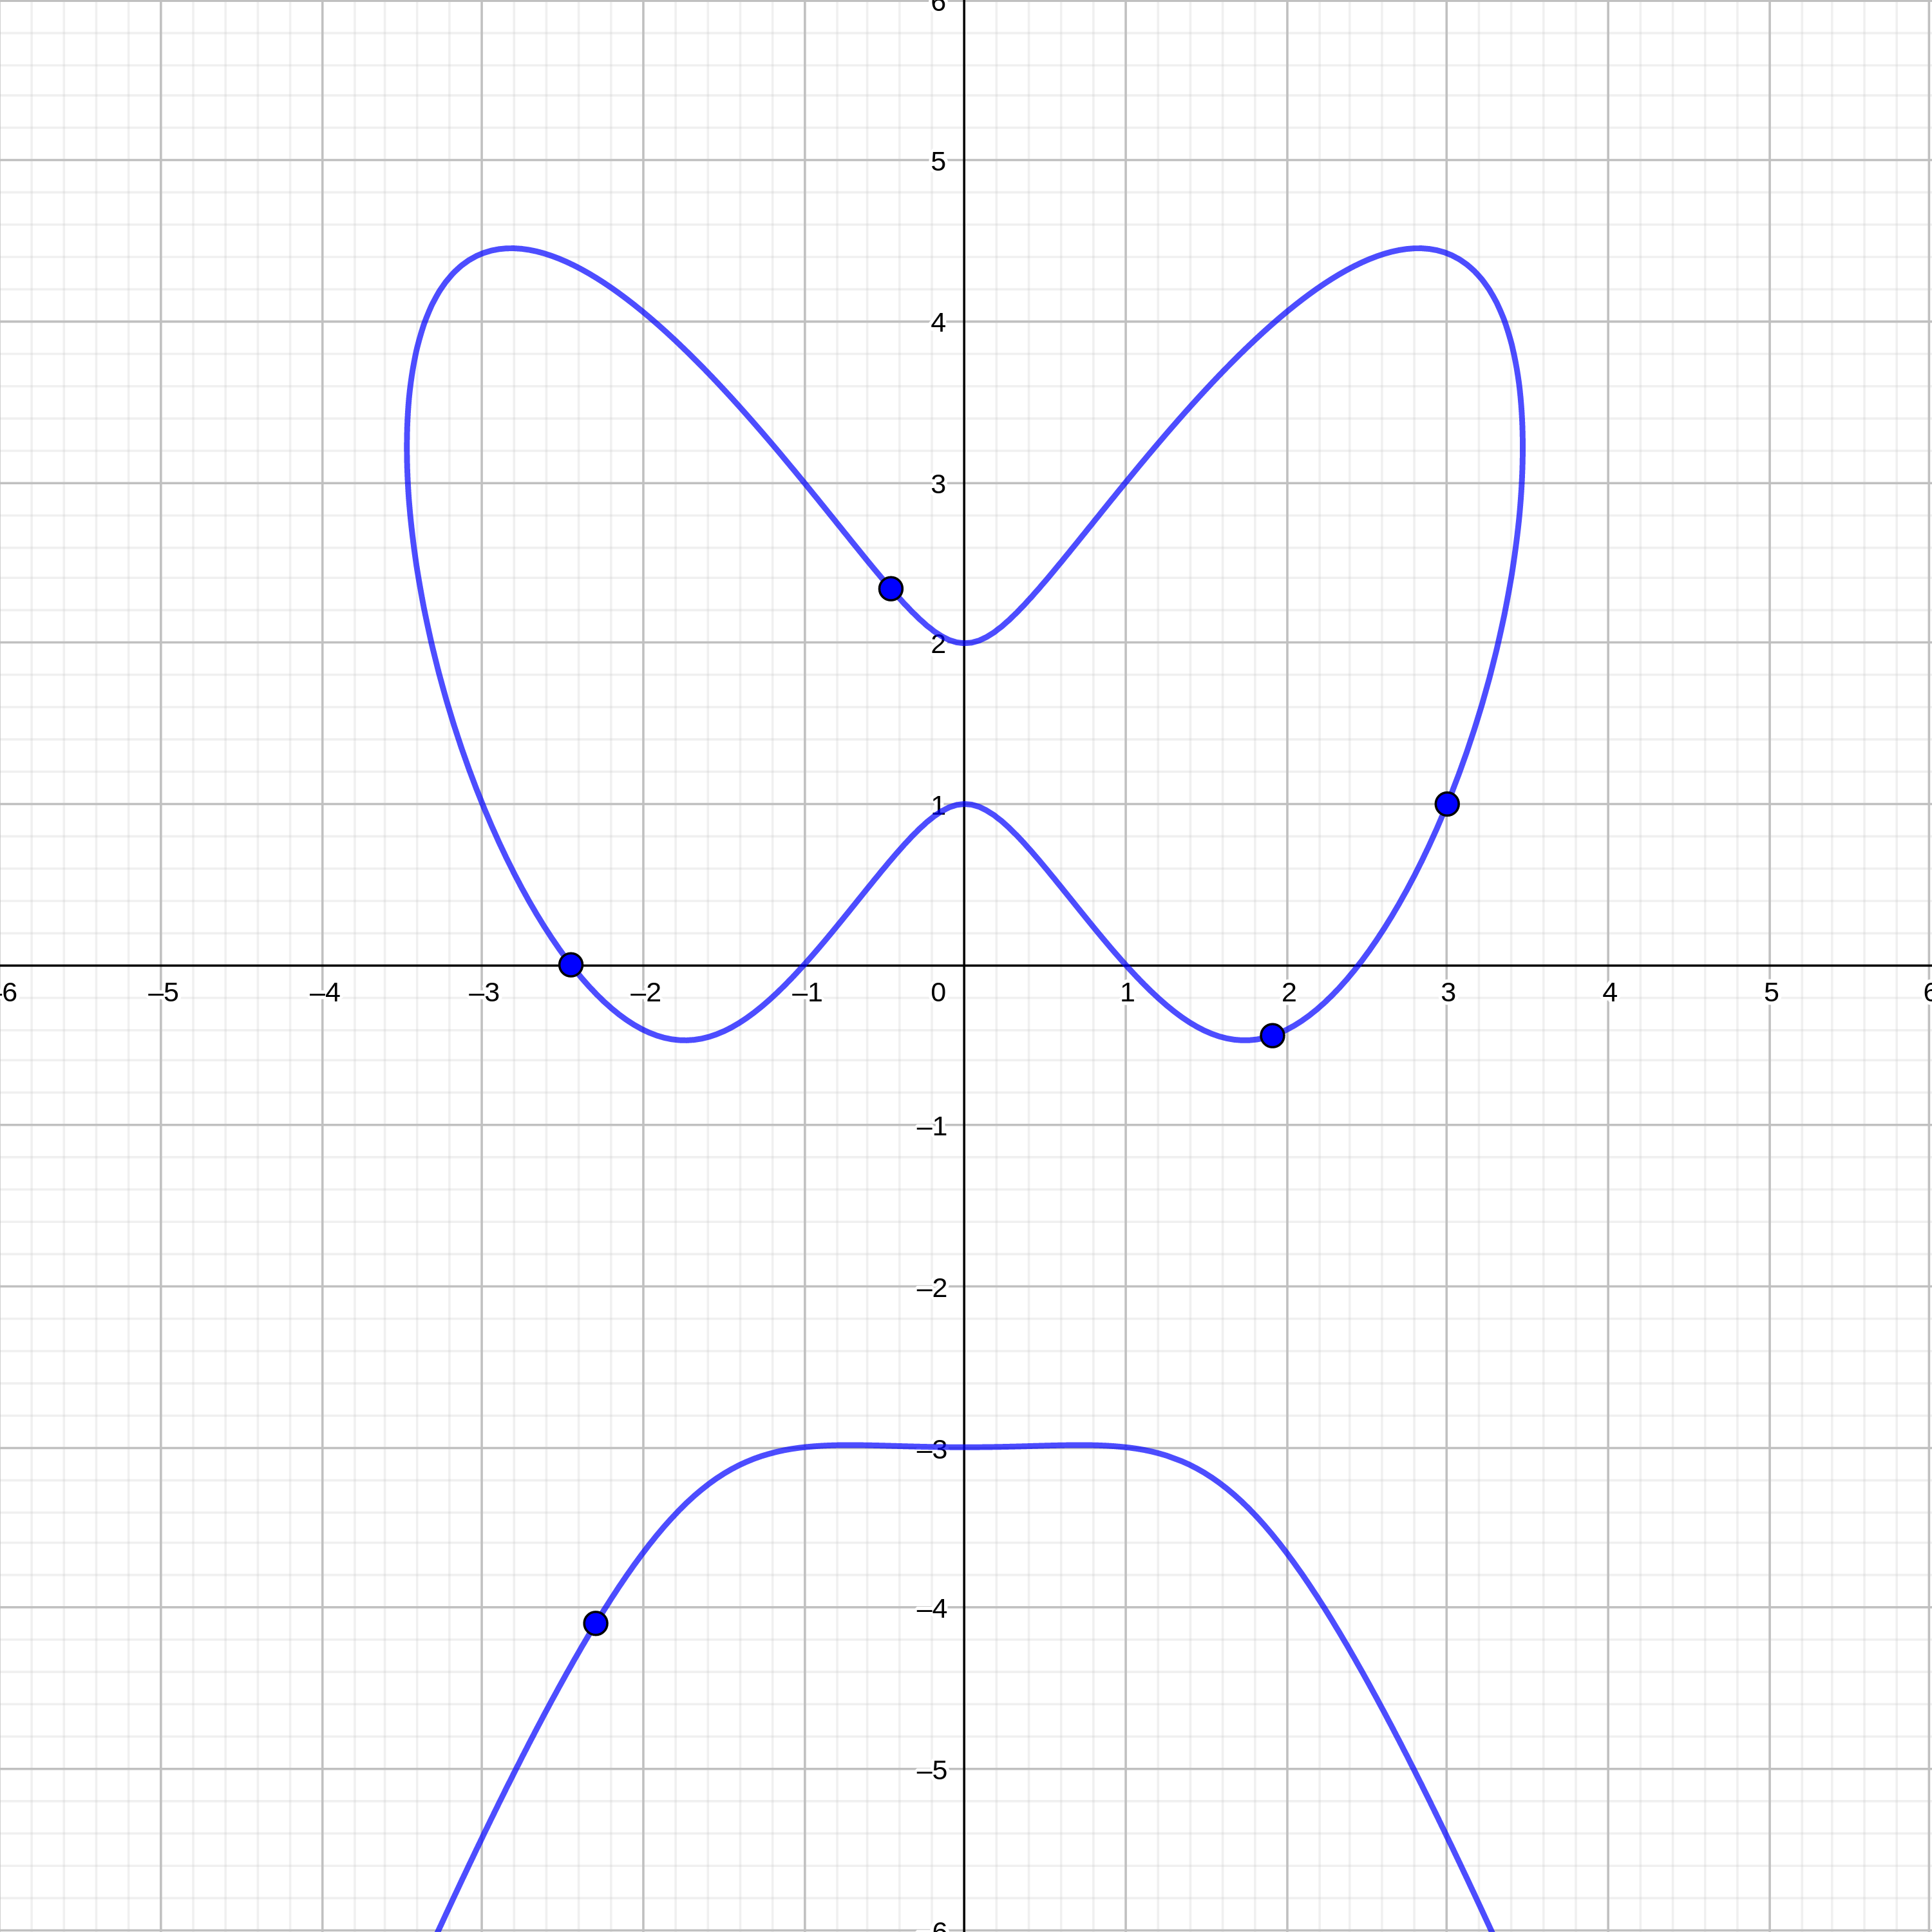
\includegraphics[height=7.6cm]{lcm_d1_d2.png} \end{center}
\end{frame}
\begin{frame}
\frametitle{$\gcd(D, D')$}
  \begin{center} 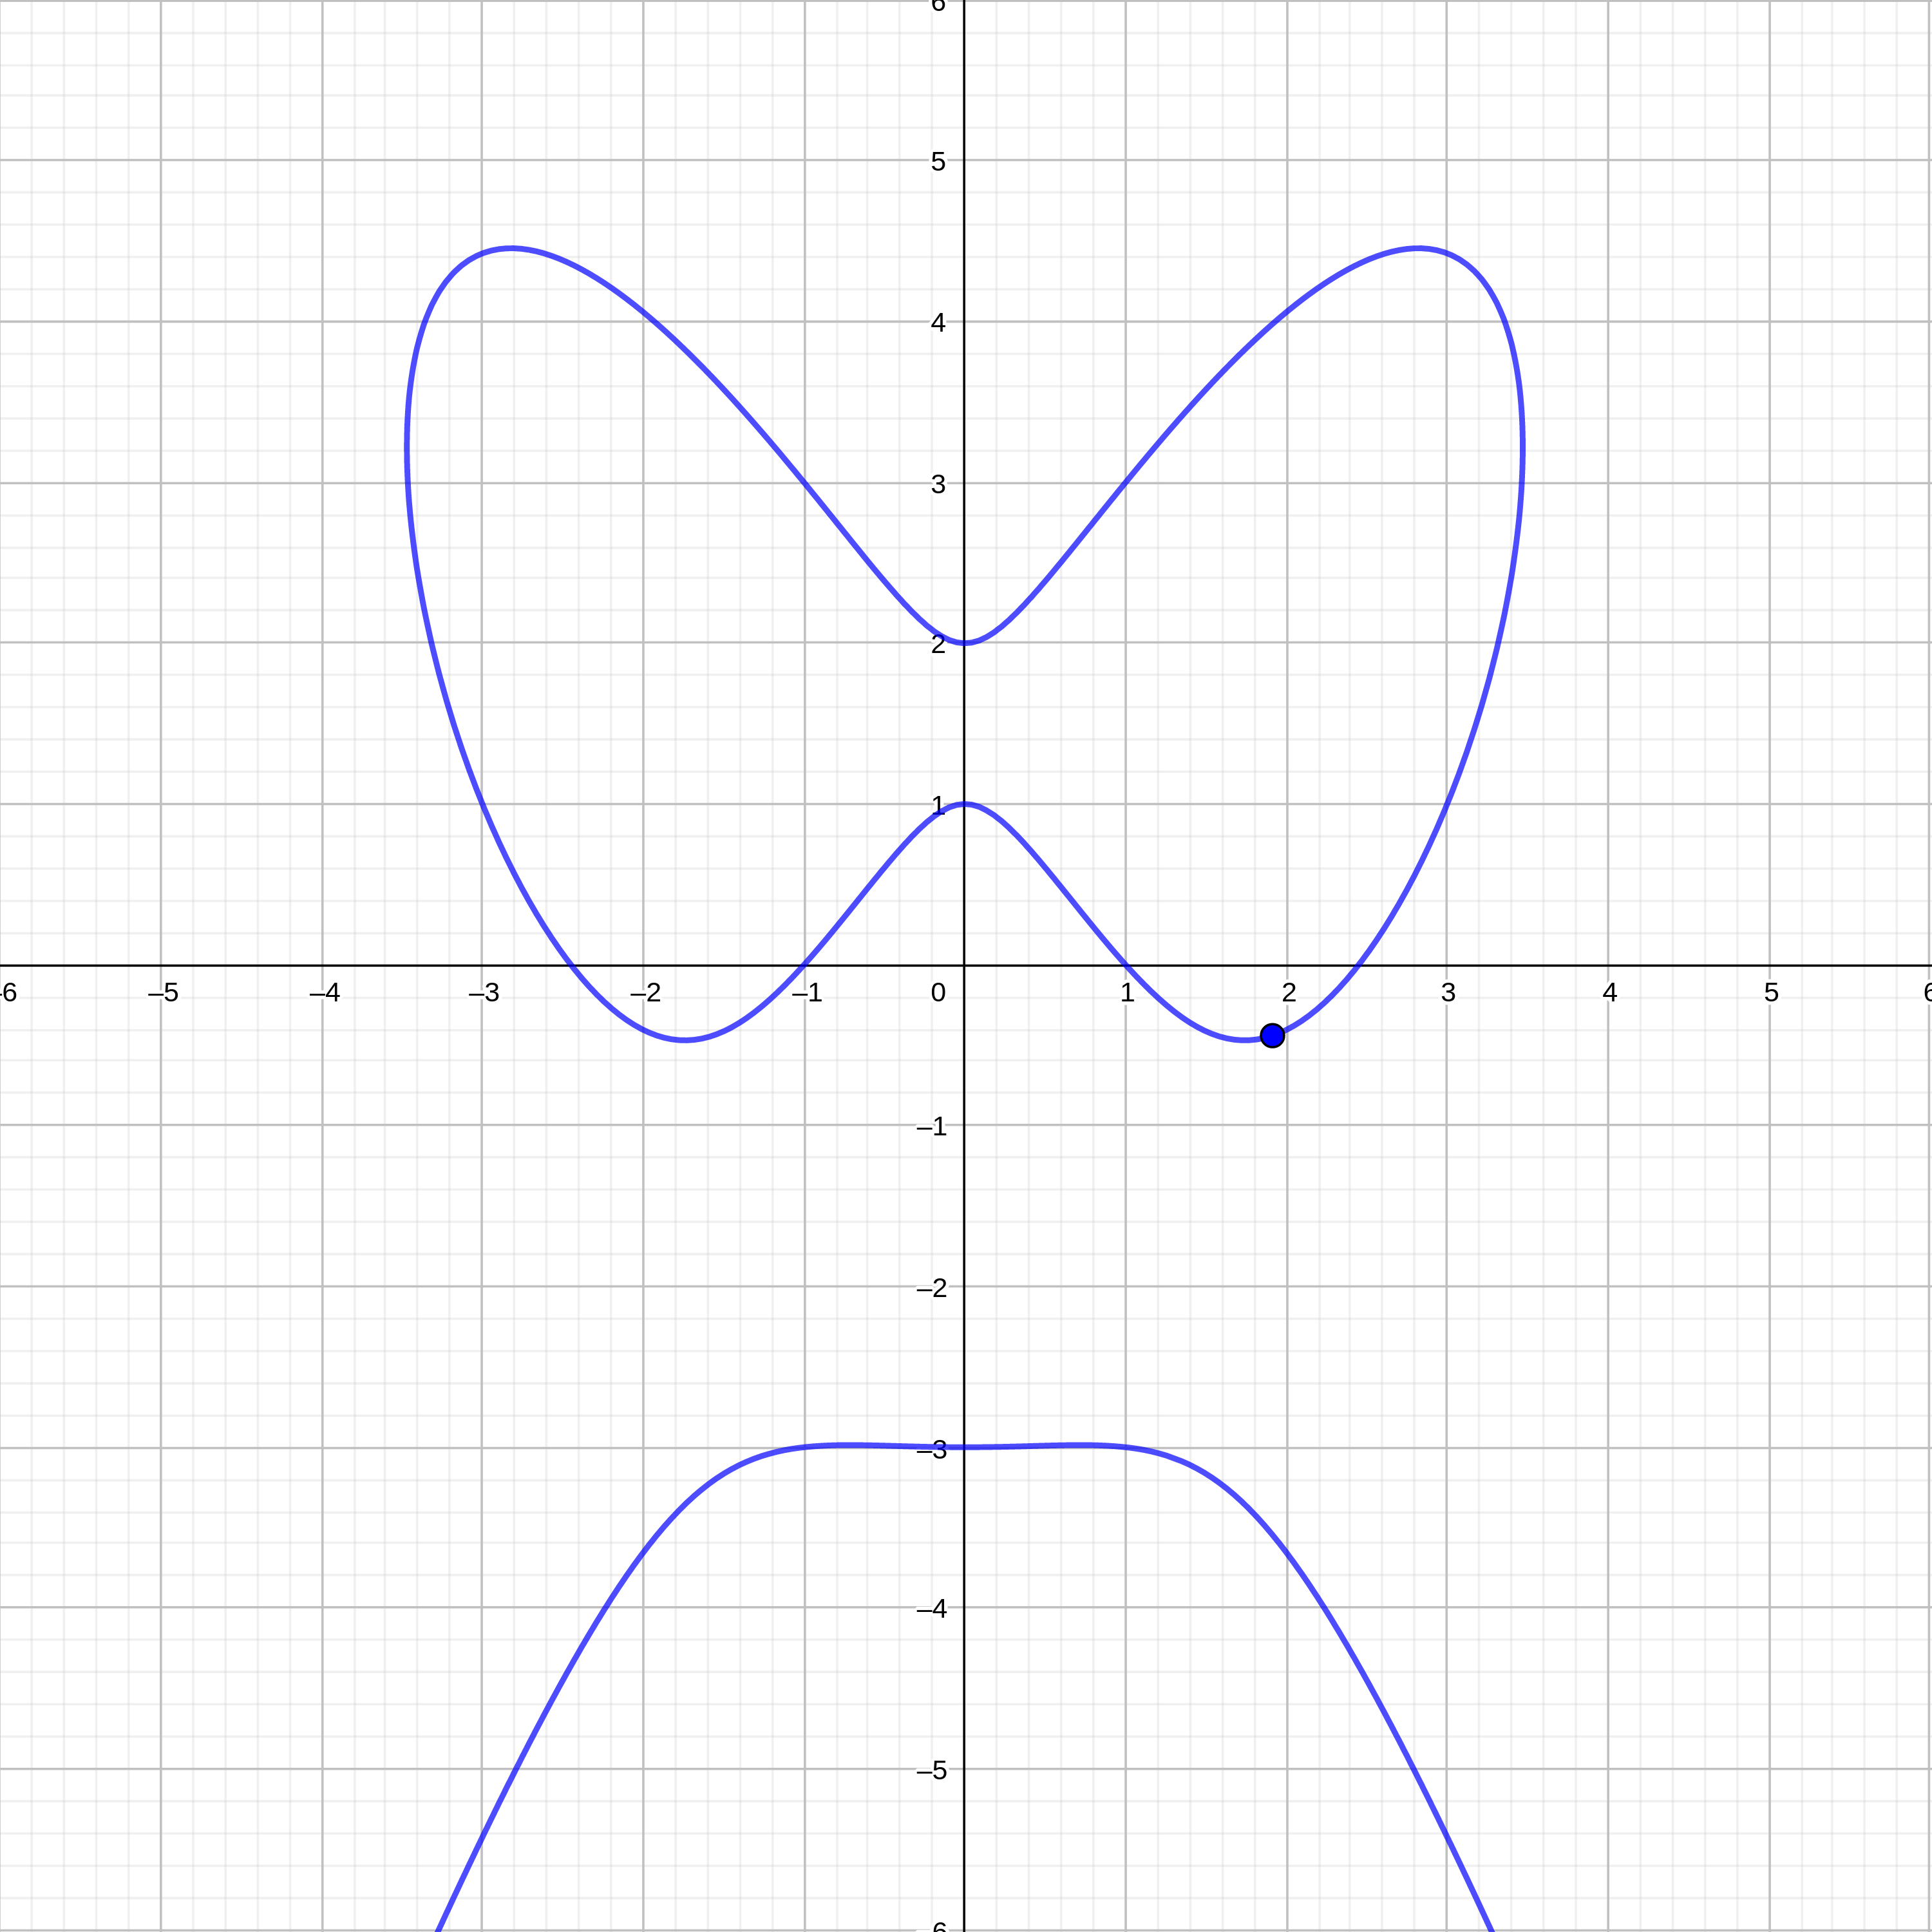
\includegraphics[height=7.6cm]{gcd_d1_d2.png} \end{center}
\end{frame}
\begin{frame}
\frametitle{$D$}
  \begin{center} 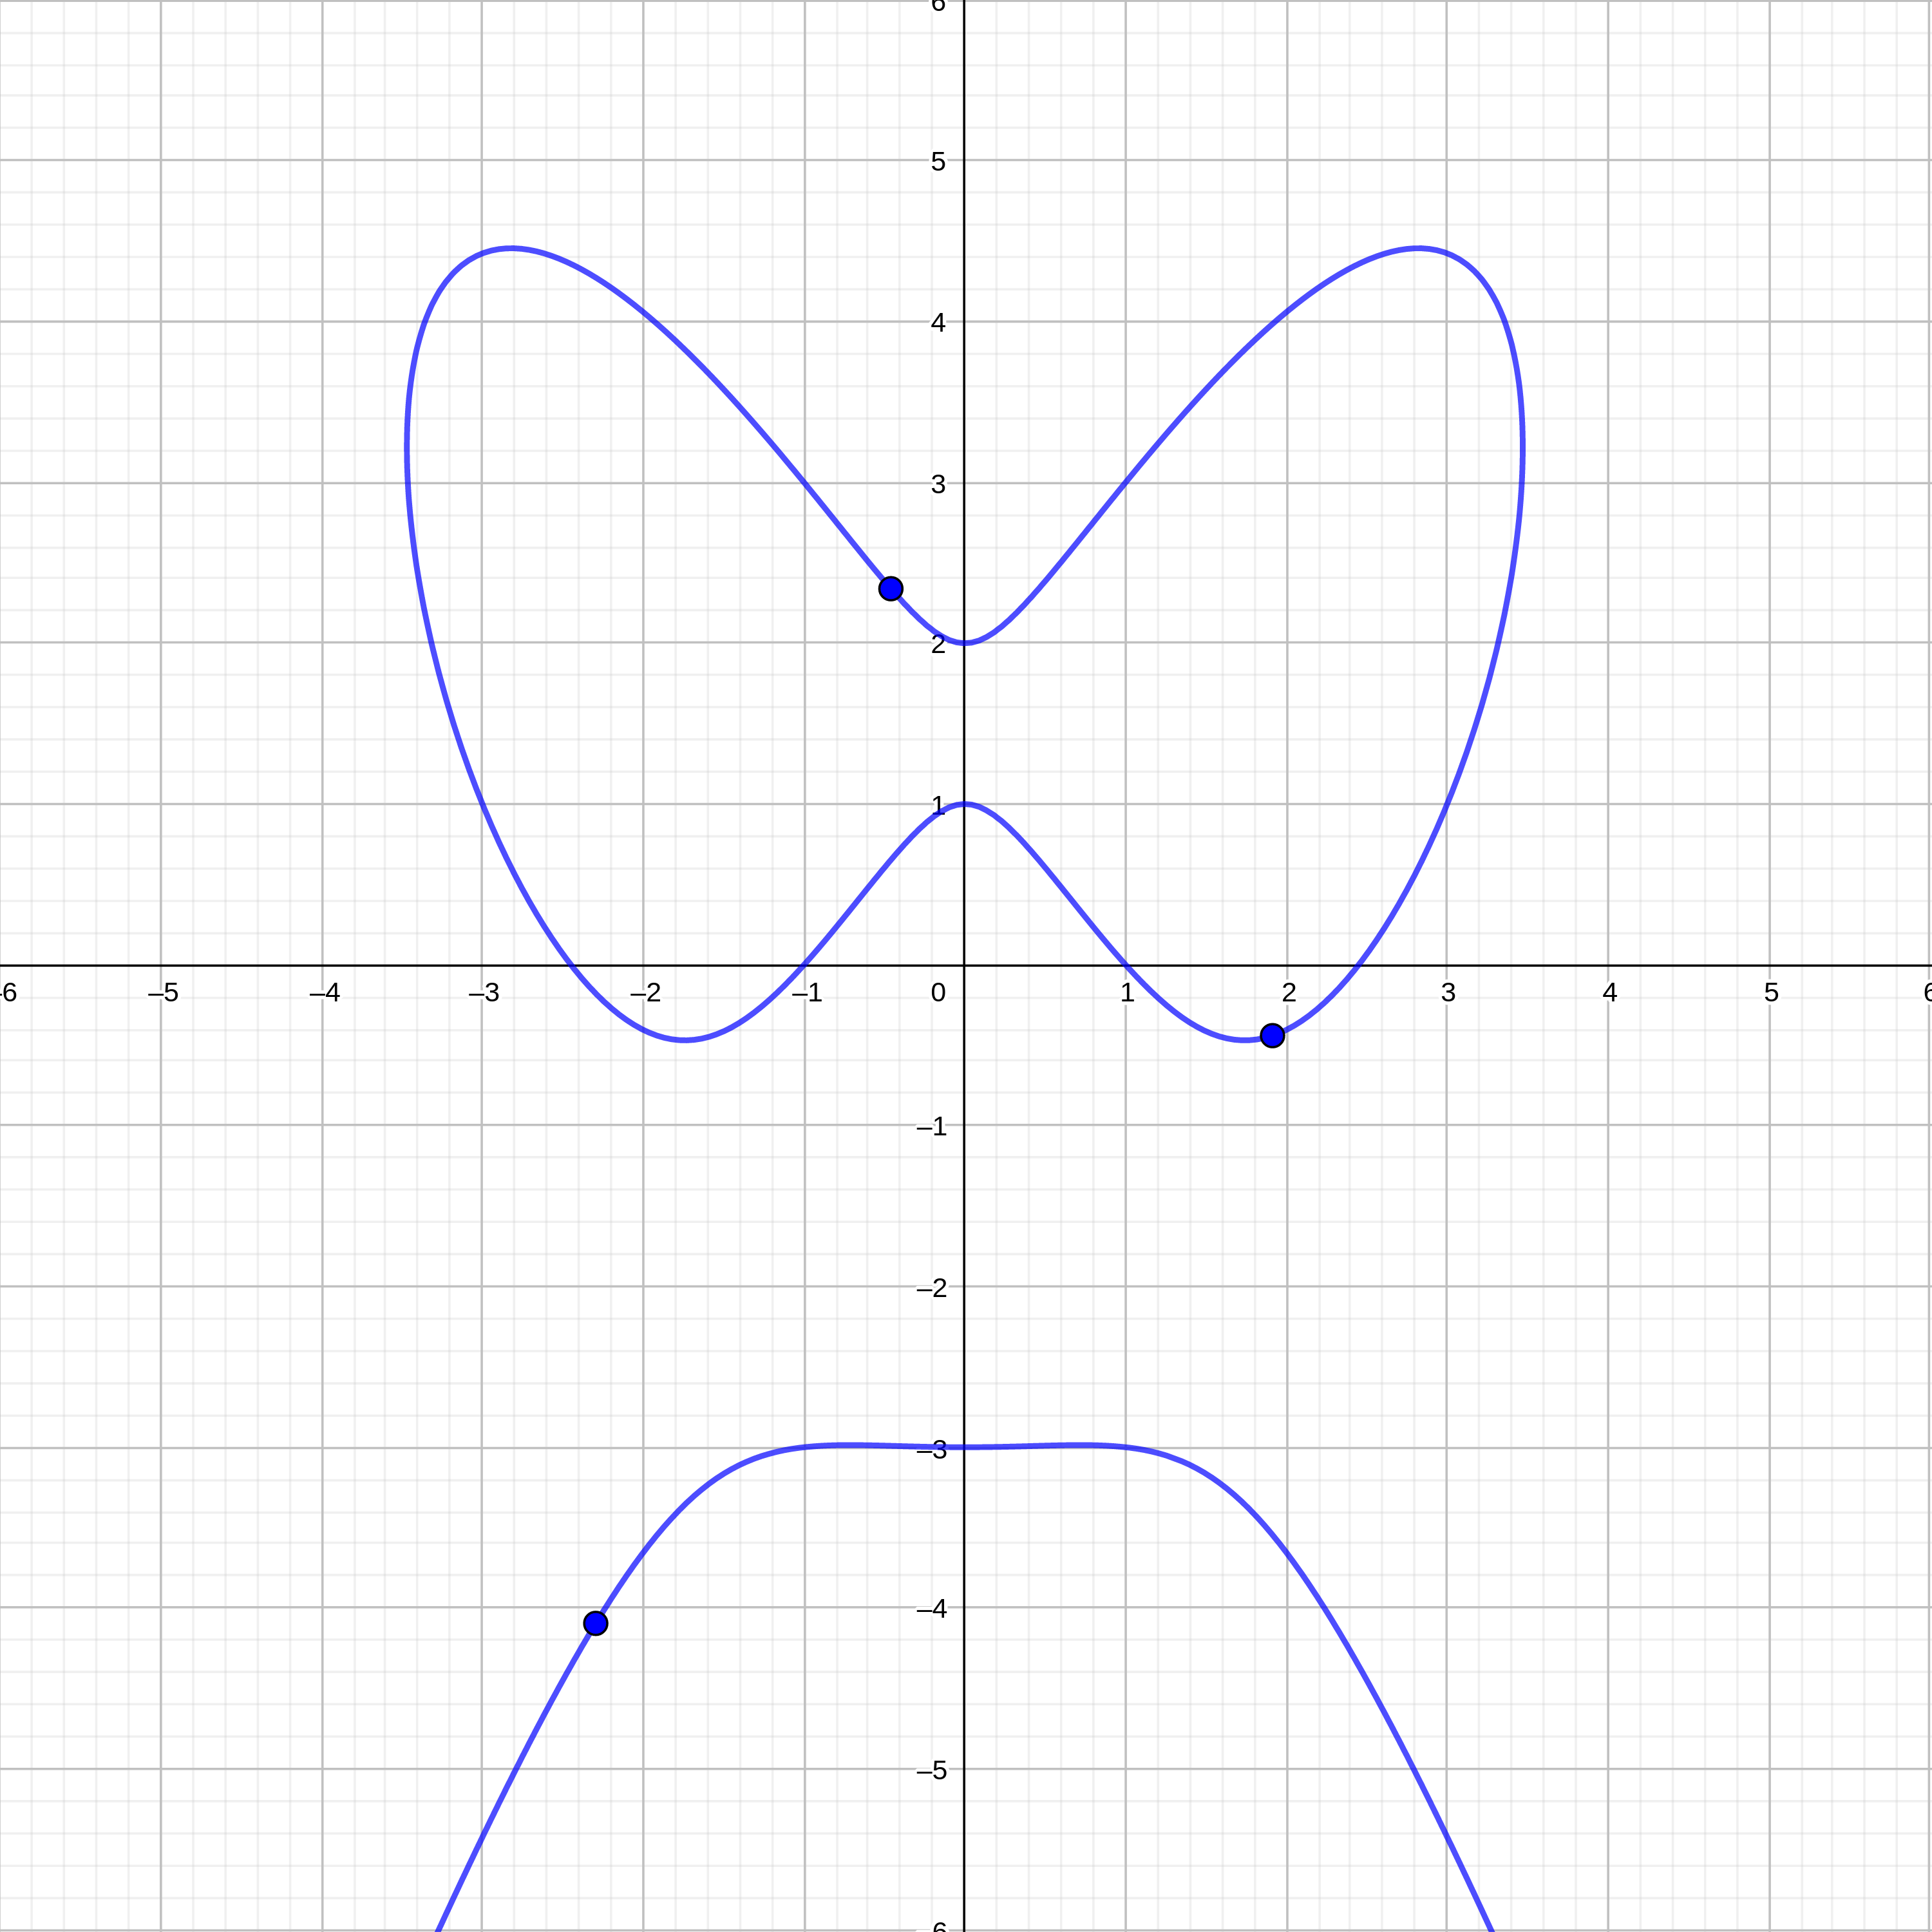
\includegraphics[height=7.6cm]{d1.png} \end{center}
\end{frame}
\begin{frame}
\frametitle{$I_D = \pid{f, g, h}$}
  \begin{center} 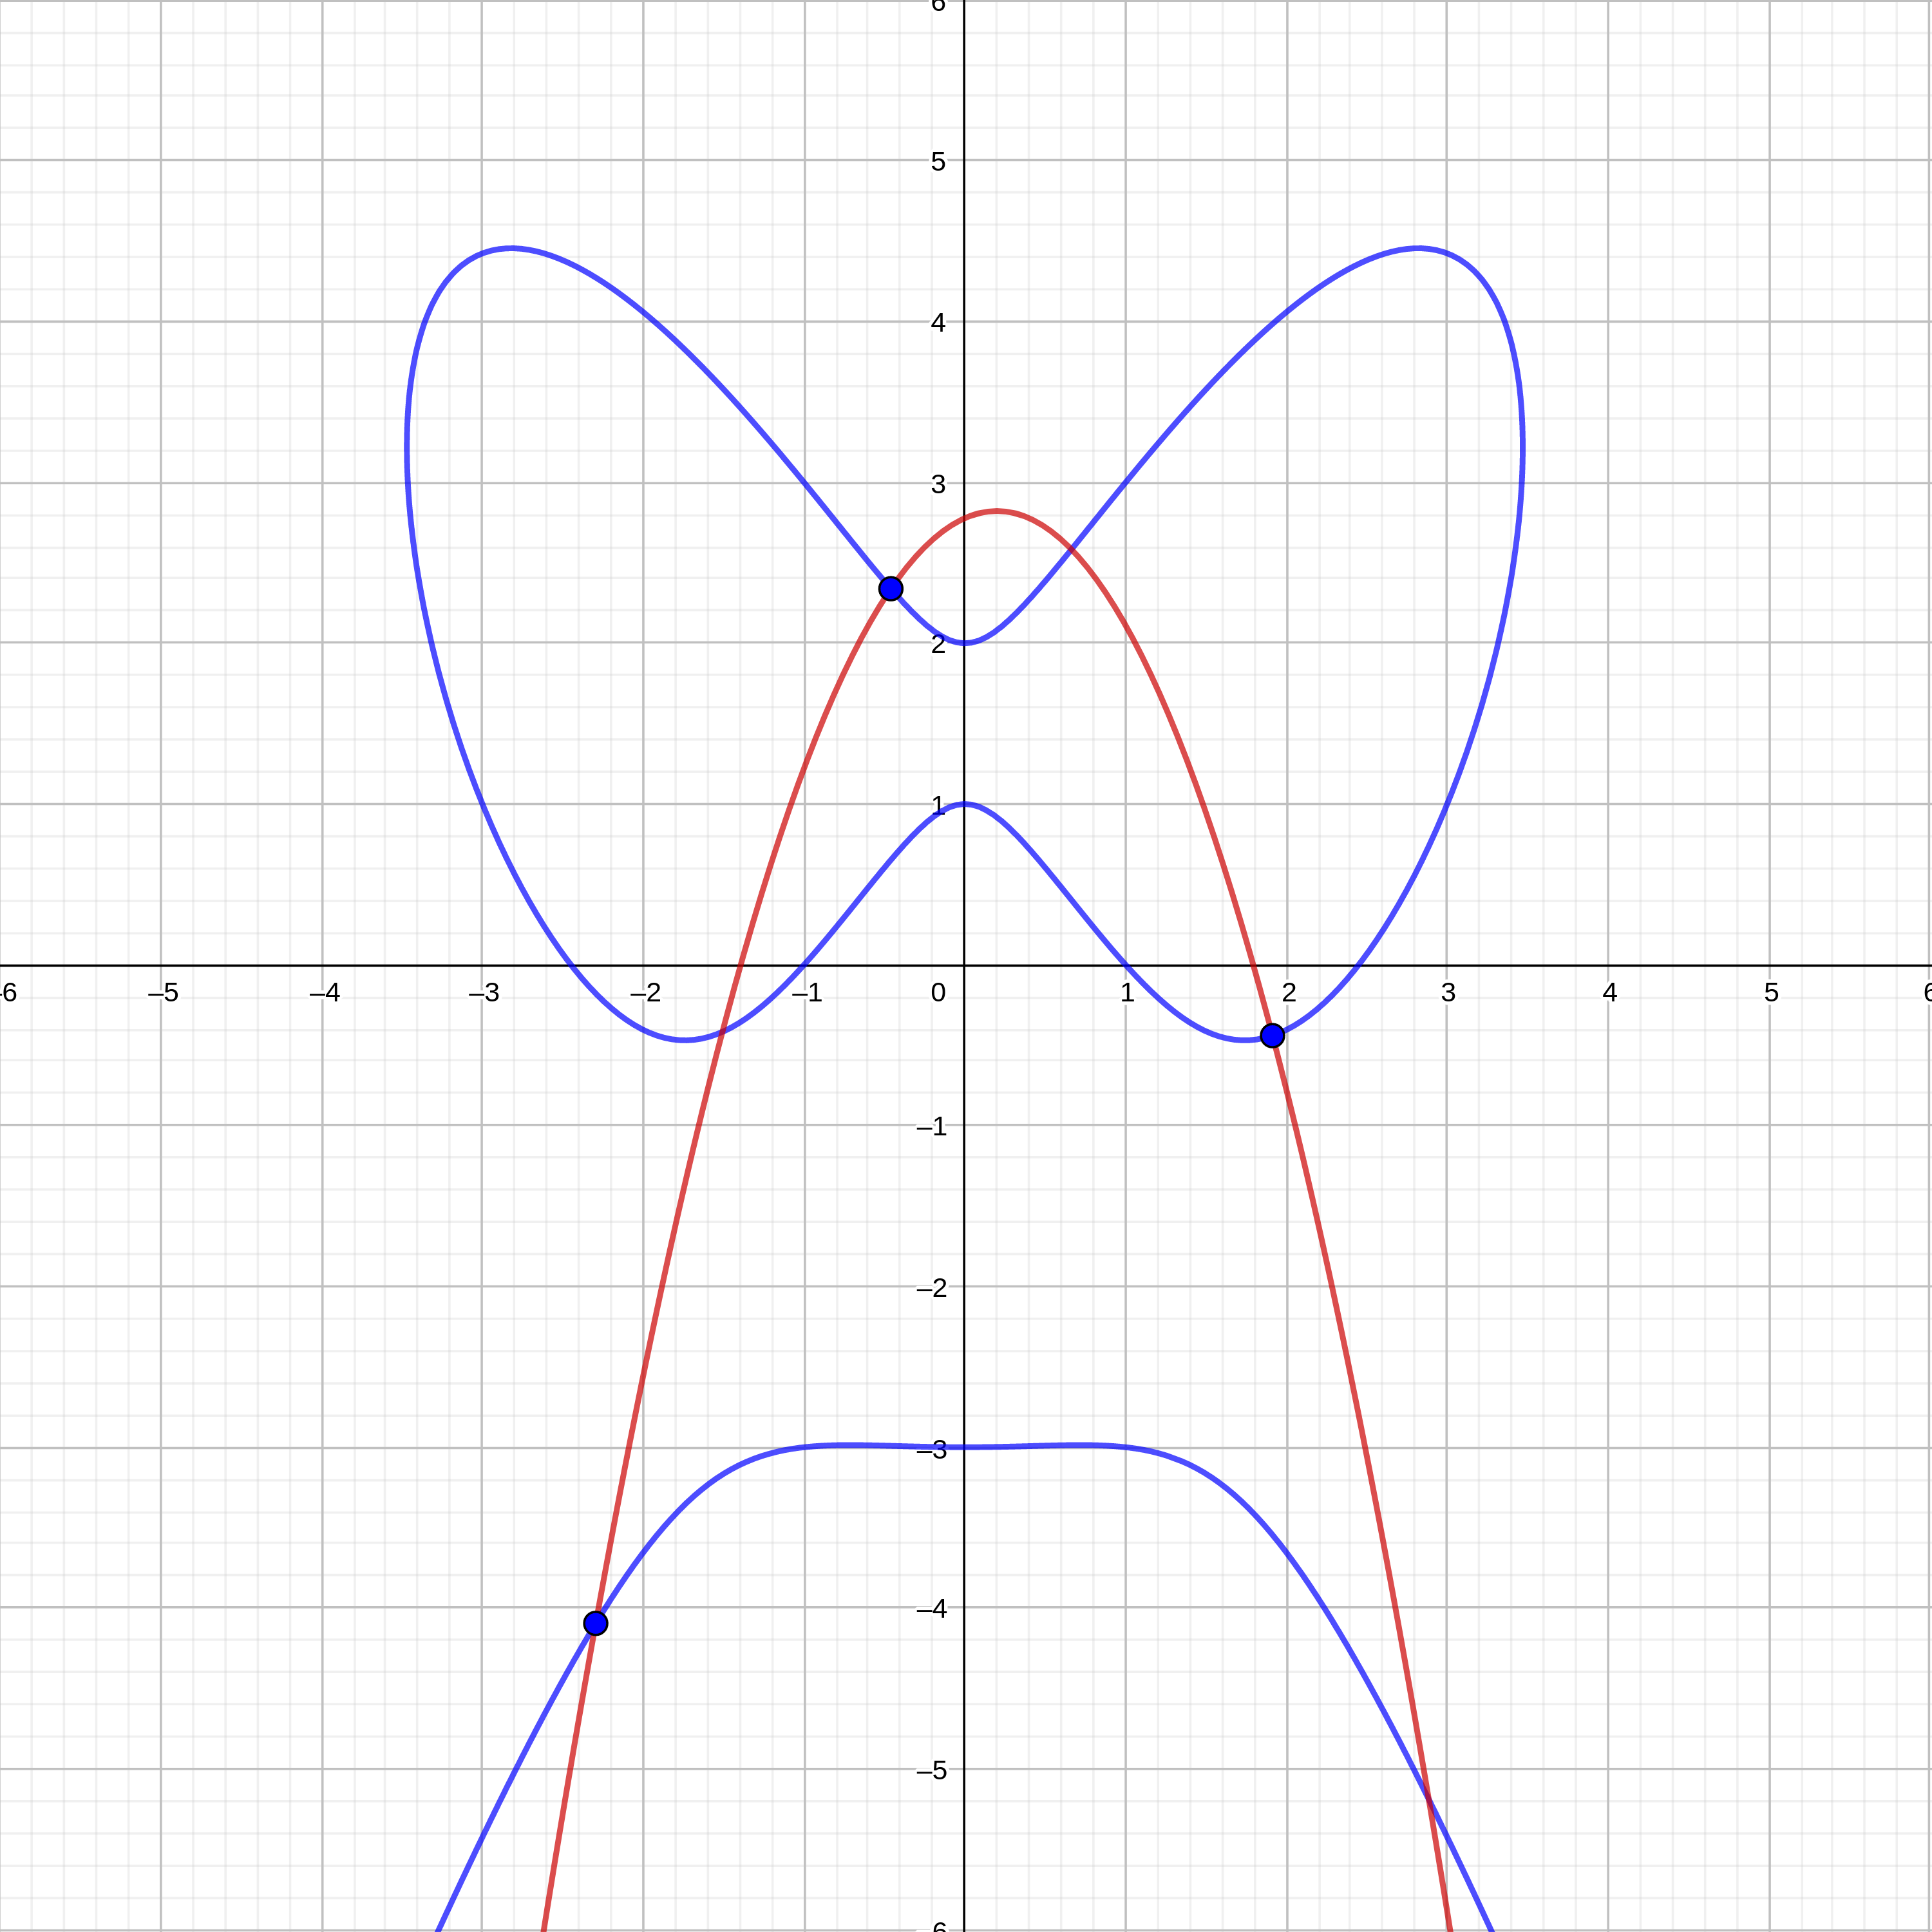
\includegraphics[height=7.6cm]{d1_f.png} \end{center}
\end{frame}
\begin{frame}
\frametitle{$\bar D \simeq f : I_D$}
  \begin{center} 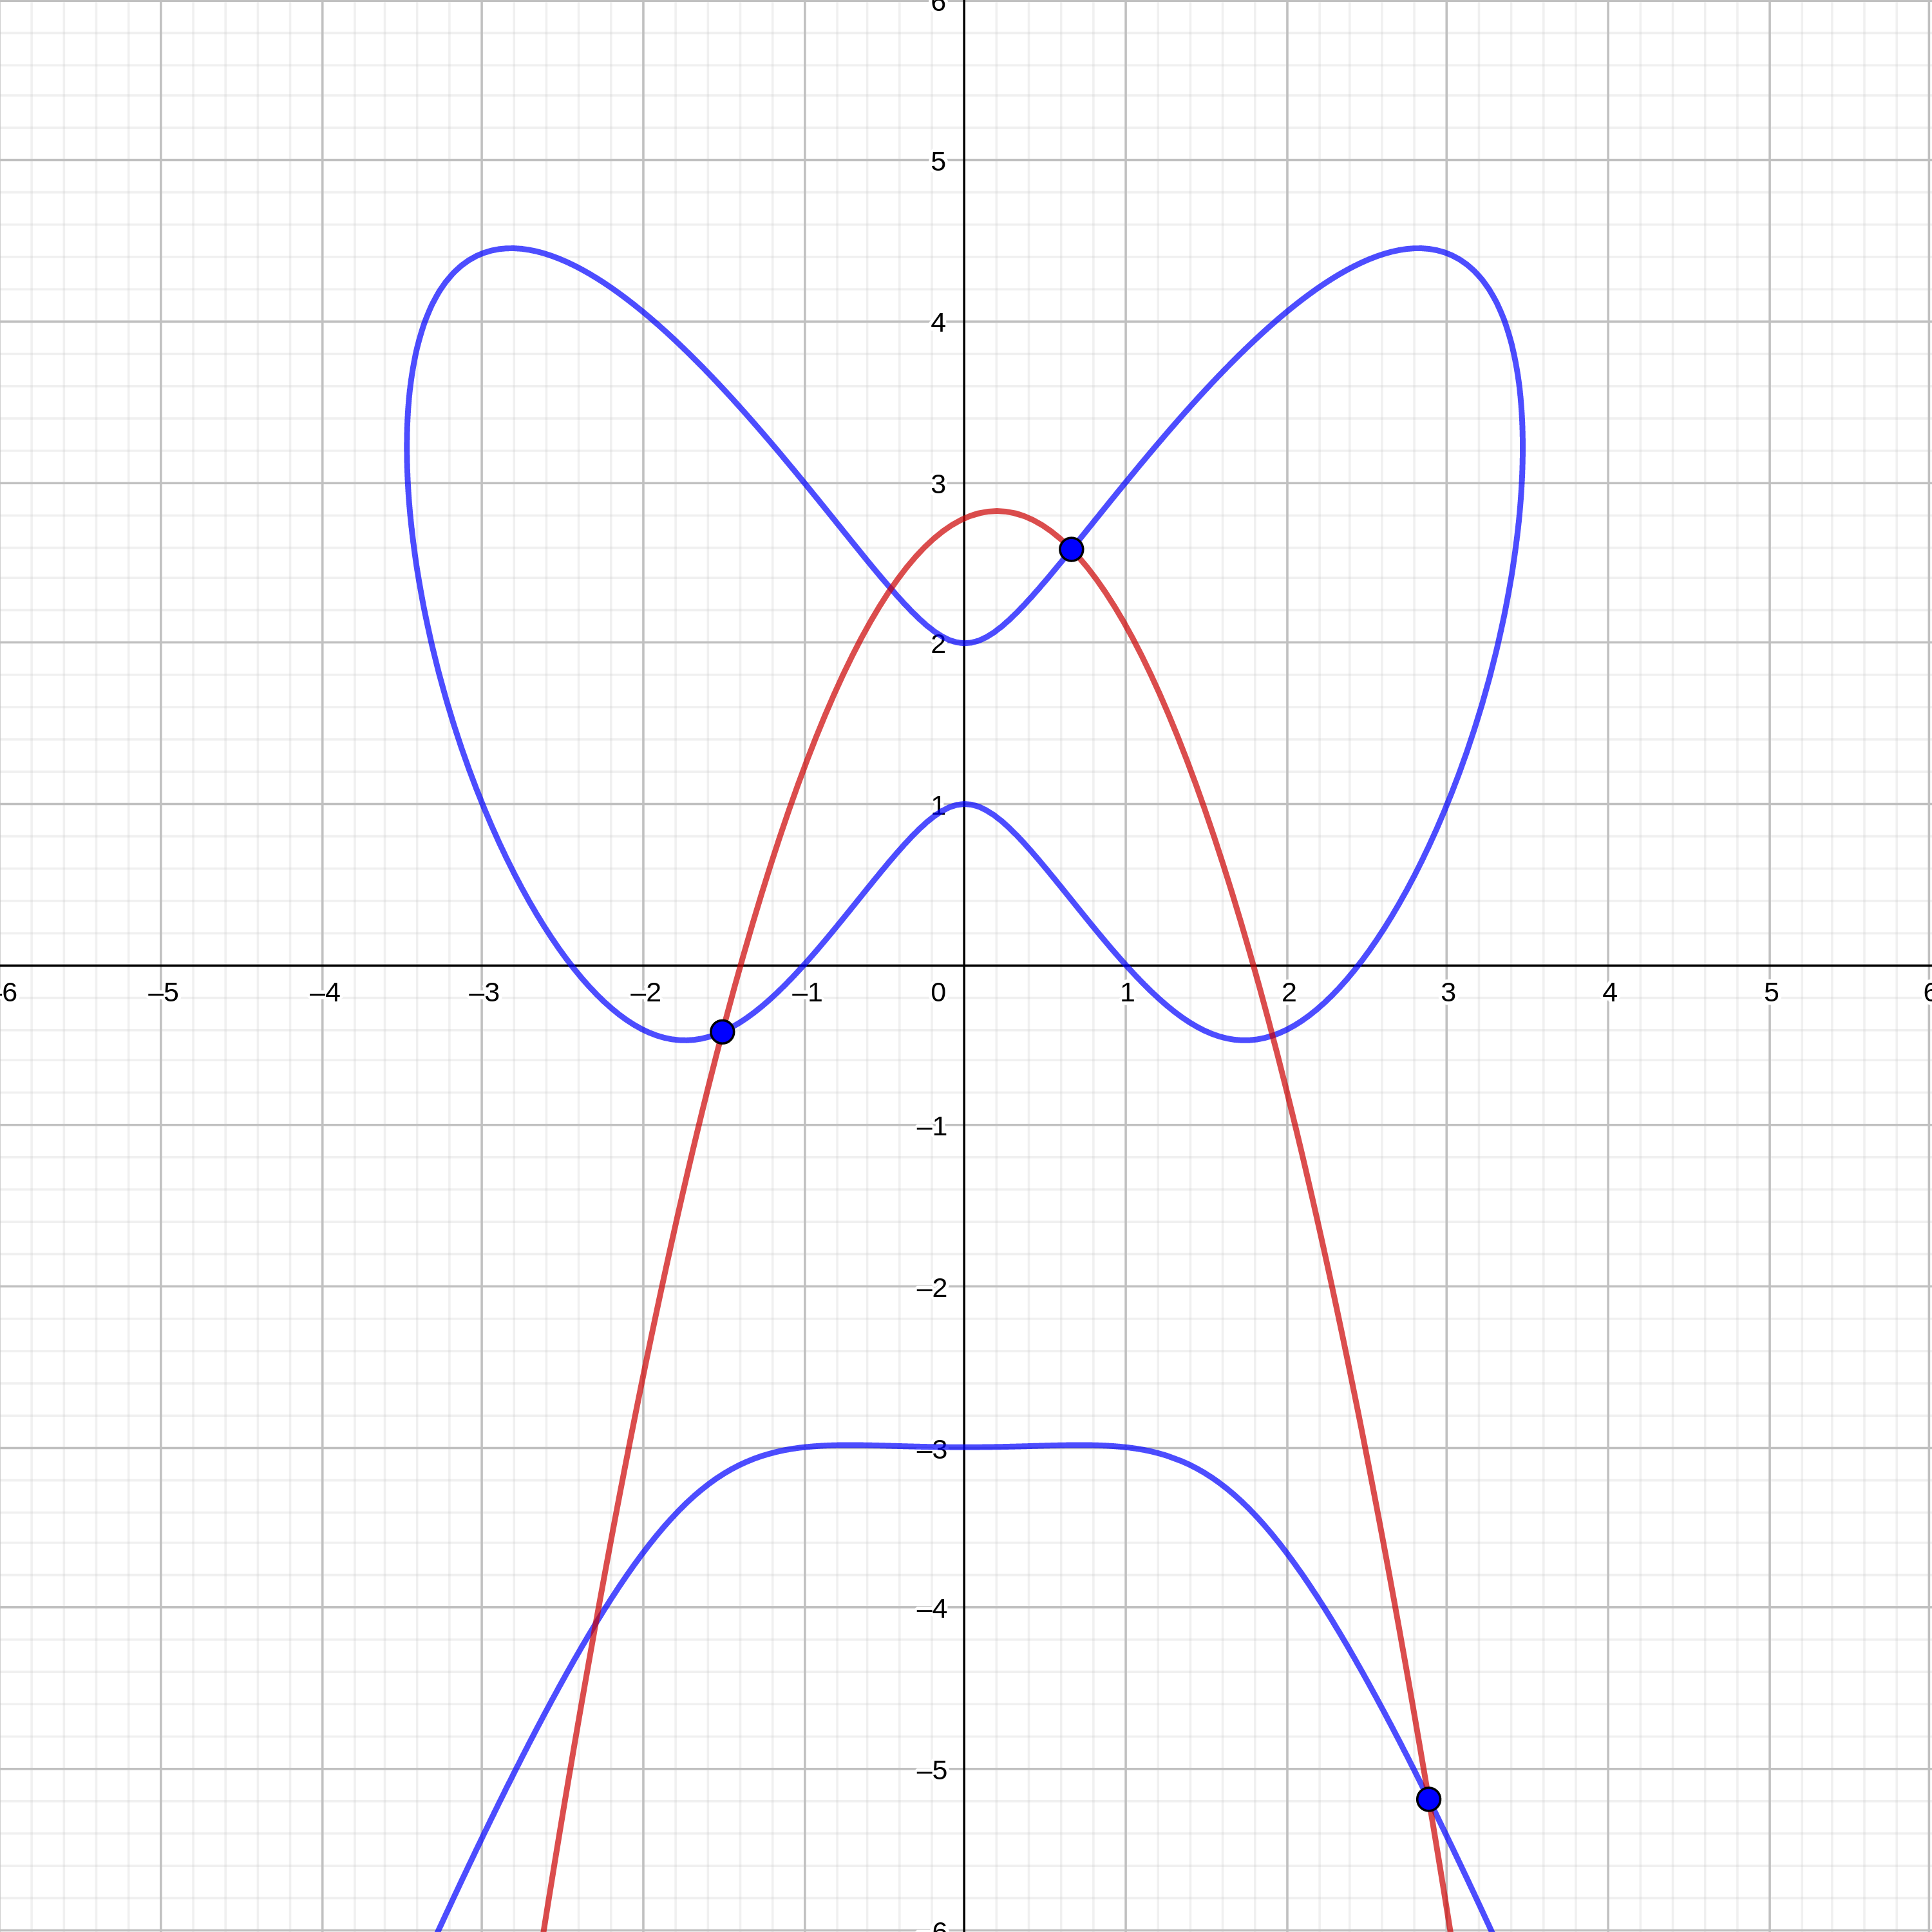
\includegraphics[height=7.6cm]{flip_d1.png} \end{center}
\end{frame}
%\end{comment}

%------------------------------------------------

\begin{frame}
\frametitle{Reduction}
  \begin{definition}
    A divisor $D$ is reduced if $\bar{\bar D} = D$.
  \end{definition}
  \begin{theorem}
    For any divisor $D$:
    \begin{enumerate}
      \item $\bar{\bar{\bar D}} = \bar D$;
      \item $\bar D \equiv -D$;
      \item $\bar{\bar D} \equiv D$;
      \item $\bar D$ and $\bar{\bar D}$ are reduced.
    \end{enumerate}
  \end{theorem}
\end{frame}

%------------------------------------------------

\begin{frame}
\frametitle{High-level Algorithm}
  Given divisors $I_D = \pid{f, g, h}, I_{D'} = \pid{f', g', h'}$,\\
  to compute a reduced divisor $I_{D''} = \pid{f'', g'', h''}$ equivalent to $D + D'$.
  \begin{enumerate}
    \item Compute a RGB $\pid{u, v, w}$ for $J = I_D I_{D'}$.
    \item Compute a RGB $\pid{u', v', w'}$ for $J^* = u : J$.
    \item Compute a RGB $\pid{f'', g'', h''}$ for $I_{D''} = u' : J^*$.
  \end{enumerate}
  \vspace{10pt}
  One can do two flips for less than the cost of one!\footcite{kamal18}
\end{frame}

%------------------------------------------------

\begin{frame}
\frametitle{Reducing to Linear Algebra}
  $I_D$ has structure as a (infinite-dimensional) $K$-vector space, $W_D$.
  \vspace{10pt}
  Polynomials in $I_D$ ``bounded'' by a monomial $m$ form a finite-dimensional vector space, $W_D^m$.
  \vspace{10pt}
  For sufficiently large $m$,
  \[ \text{$I_D$'s reduced Gr\"obner basis} \subseteq \text{$W_D^m$'s reduced echelon basis}. \]
\end{frame}

%------------------------------------------------

\begin{frame}[fragile]
\frametitle{Framework for Addition}
  \note{describe where kamal's work ends}
  \begin{center}
    \begin{tikzcd}
      W_L^m \arrow[hook]{r}{\ker M} &
      W_D^m \arrow[hook]{r}{\iota} \arrow[bend left]{rr}{M} & 
      W_0^m \arrow[two heads]{r}{\pi} & 
      \frac {W_0^m} {W_{D'}^m} \arrow[two heads]{r}{\im M} & 
      \frac {W_G^m} {W_{D'}^m}
    \end{tikzcd}
  \end{center}
  $M$ is reduction of $W_D^m$ modulo $W_{D'}^m$.\\
  \vspace{10pt}
  $L := \lcm(D, D')$ is recovered from $\ker M$.\\
  $G := \gcd(D, D')$ is recovered from $\im M$.\\
  \vspace{10pt}
  In general $D + D' = L + G$. Return\\
  %When $D$ and $D'$ are disjoint, $D + D' = L$ and $G = 0$.\\
  %\vspace{10pt}
  %Compute $L$, $G$ (if necessary), and return \[D + D' = \bar{\bar L} + G.\]
  \[D + D' = \bar{\bar L} + G.\]
\end{frame}

%------------------------------------------------

\begin{comment}
\begin{frame}[fragile]
\frametitle{Framework for Addition}
  Given divisiors $D$ and $D'$, \\
  to compute a (not necessarily reduced) divisor equivalent to $D + D'$
  \begin{enumerate}
    \item Compute $M$ and its RREF. \\
    \item If $M$ has full rank, return $L$. \\
    \item Otherwise, if $\rank M > 0$, return $\bar{\bar L} + G$. (Recursion).\\
    \item When $\rank M = 0$, find $D''$ and largest $n$ such that $D = D'' + nD'$.\\
          Return $D'' + \bar{\bar{(n + 1)D'}}$.
  \end{enumerate}
  The last step requires computing scalar multiples \\
  $2D', 3D'\sout[red]{, 4D', 5D', 6D'}.$\\
\end{frame}
\end{comment}

%------------------------------------------------

\begin{comment}
\begin{frame}[fragile]
\frametitle{Addition Example}
  Let $C : y^3 + x^4 + 1$ be a $C_{3,4}$ curve over $\bb F_{11}$.
  Let $D$ and $D'$ be divisors with
  \begin{align*}
    I_D &= \pid{f, g, h}     & I_{D'} &= \pid{f', g', h'} \\
    f   &= x^2 + 3y + 7x + 5 & f'     &= x^2 + 6y + 3x - 2 \\
    g   &= xy + 2y + 2x + 9  & g'     &= xy + 5y + 5x + 9 \\
    h   &= y^2 + 4y + 2x + 3 & h'     &= y^2 - y - x + 5.
  \end{align*}
\end{frame}

%------------------------------------------------

\begin{frame}[fragile]
\frametitle{Addition Example}
  \[W_D^{x^4} = \Span\{ f, g, h, xf, xg, xh, x^2f \} \]
  \[W_{D'}^{x^4} = \Span\{ f', g', h', xf', xg', xh', x^2f' \} \]
  Compute $f, g, h, \dots$ modulo $f', g', h', \dots$. E.g.
  \begin{align*}
    \bar f &= f - f' \\ &= {\color{red}8}y + {\color{red}4}x + {\color{red}7}
  \end{align*}
  \[ M = \begin{pmatrix}
    {\color{red}7} & 0 & 9 & 2 & 10 & 5 & 2 \\
    {\color{red}4} & 8 & 3 & 10 & 2 & 8 & 6 \\
    {\color{red}8} & 8 & 5 & 2 & 0 & 1 & 7
  \end{pmatrix} \]
\end{frame}

%------------------------------------------------

\begin{frame}[fragile]
\frametitle{Addition Example}
  \[ M_{\text{rref}} = \begin{pmatrix}
    1 & 0 & 6 & 0 & 6 & 9 & 2 \\
    0 & 1 & 7 & 0 & 9 & 8 & 10 \\
    0 & 0 & 0 & 1 & 6 & 4 & 5
  \end{pmatrix} \]
  \[ \ker M =
  \begin{pmatrix}
    -6 & -6 & -9 & -2 \\
    -7 & -9 & -8 & -10 \\
     1 &  0 &  0 &  0 \\
     0 & -6 & -4 & -5 \\
     0 &  1 &  0 &  0 \\
     0 &  0 &  1 &  0 \\
     0 &  0 &  0 &  1
  \end{pmatrix} \]
  \[ I_L = \pid{ \begin{array}{l}
      h - 7g - 6f, \\
      xg - 6xf - 9g - 6f, \\
      xh - 4xf - 8g - 9f, \\
      x^2f - 5xf - 10g - 2f \end{array} } \]
\end{frame}

%------------------------------------------------

\begin{frame}[fragile]
\frametitle{Addition Example}
  \begin{align*}
    I_L &=
      \pid{ \begin{array}{l}
        h - 7g - 6f, \\
        xg - 6xf - 9g - 6f, \\
        xh - 4xf - 8g - 9f, \\
        x^2f - 5xf - 10g - 2f
      \end{array} } \\
      &= \pid{ \begin{array}{l}
        y^2 + 4xy + 5x^2 + 5y + x - 2, \\
        x^2y + 5x^3 - 3xy - 2x^2 - 3y - 4x - 1, \\
        \sout[red]{xy^2 - 4x^3 - 5xy - 2x^2 + y + 3x + 4}, \\
        \sout[red]{x^4 + 3x^2y + 2x^3 - 3xy + x^2 - 4y - 4x - 1}
      \end{array} }
  \end{align*}
\end{frame}
\end{comment}

%------------------------------------------------

\begin{frame}
\frametitle{Explicit Formulas}
  Adding two typical divisors $I_D = \pid{f,g,h}$ and $I_{D'} = \pid{f',g',h'}$:
  \begin{align*}
    I_D &= \pid{f, g, h}           & I_{D'} &= \pid{f', g', h'} \\
    f   &= x^2 + f_2y + f_1x + f_0 & f'     &= x^2 + f'_2y + f'_1x + f'_0 \\
    g   &=  xy + g_2y + g_1x + g_0 & g'     &=  xy + g'_2y + g'_1x + g'_0 \\
    h   &= y^2 + h_2y + h_1x + h_0 & h'     &= y^2 + h'_2y + h'_1x + h'_0
  \end{align*}
  \[ M = \begin{pmatrix}
    a_1 & a_2 & \dots & a_7 \\
    a_8 & a_9 & \dots & a_{14} \\
    a_{15} & a_{16} & \dots & a_{21}
  \end{pmatrix} \]
  \begin{align*}
    a_1    &= f_0 - f'_0 & \dots && a_7    &=     - f'_0a_{11} - g'_0a_{18} \\
    a_8    &= f_1 - f'_1 & \dots && a_{14} &= a_4 - f'_1a_{11} - g'_1a_{18} \\
    a_{15} &= f_2 - f'_2 & \dots && a_{21} &=     - f'_2a_{11} - g'_2a_{18}
  \end{align*}
\end{frame}

%------------------------------------------------

\begin{frame}
\frametitle{Explicit Formulas}
  \[ \ker M = \begin{pmatrix}
    r_0 & r_1 & r_2 & 1 & 0 & 0 & 0 \\
    s_0 & s_1 & s_2 & 0 & 1 & 0 & 0 \\
    t_0 & t_1 & t_2 & 0 & 0 & 1 & 0 \\
      * &   * &   * & 0 & 0 & 0 & 1
  \end{pmatrix}^T \]
  Write $r_i, s_i, t_i$ in terms of $a_i$. \\
  Then $I_L = \pid{u, v, w}$ where, e.g.
  \begin{align*}
    u &= x^3 + u_5y^2 + u_4xy + \dots + u_0 \\
    u_5 &= r_2 \\
    u_4 &= r_1 + f_2 \\
    \vdots \\
    u_0 &= f_0r_0 + g_0r_1 + h_0r_2
  \end{align*}
  Can compute $u, v, w$ in 1I 98M 71A.
\end{frame}

%------------------------------------------------

\begin{frame}[fragile]
\frametitle{Framework for Doubling}
  \begin{center}
    \begin{tikzcd}
      W_{D_1}^m \arrow[hook]{r}{\ker M} & 
      W_D^m \arrow{r}{d} \arrow[bend left]{rr}{M} & 
      W_0^{m'} \arrow[two heads]{r}{\pi} & 
      \frac {W_0^{m'}} {W_D^{m'}} \arrow[two heads]{r}{\im M} & 
      \frac {W_{D_0}^{m'}} {W_D^{m'}}
    \end{tikzcd}
  \end{center}
  $d$ sends a polynomial to its differential
  \[ d : f \mapsto df = f_xdx + f_ydy \equiv \phi \cdot \omega \pmod{dF} \]
  $D_1$ is such that $D < D_1 \leq 2D$. \\
  $D_0$ is such that $0 \leq D_0 < D$. \\
  In general $2D = D_0 + D_1$. \\
  Typically, $D_1 = 2D$ and $D_0 = 0$.
\end{frame}

%------------------------------------------------

\begin{frame}
\frametitle{Reduction}
  \begin{theorem}[Khuri-Makdisi, 2018]
    Suppose $D + D'$ is a typical degree 6 divisor with $I_{D + D'} = \pid{u,v}$.
    There exist polynomials
    \begin{align*}
      f'' &= x^2 + f_2y + f_1x + f_0 \\
      g'' &= xy + g_3x^2 + g_2y + g_1x + g_0
    \end{align*}
    such that $f''v \equiv g''u \pmod F$ and
    \[ I_{\bar{\bar{D + D'}}} = \pid{f'', g'' \text{ mod } f''}. \]
  \end{theorem}
  This can be generalized to all divisor types.
\end{frame}

%------------------------------------------------

\begin{comment}
\begin{frame}[fragile]
\frametitle{Proof Sketch}
  \[ f'' \in u : v \iff \exists t : f''v \equiv tu \pmod C \]
  \vspace{10pt}
  \begin{tikzcd}[column sep = 0pt]
    & D'' = D + D' \arrow{dl} \arrow{dr} & & & \pid{u,v} \arrow{dl} \arrow{dr} \\
    \bar{D''} \arrow{d} & & A \equiv \bar{D''} \arrow{d} & u : v = \pid{f'', g_0} \arrow{d} & & \pid{t, h_0} = v : u \arrow{d} \\
    \bar{\bar{D''}} \arrow[equal]{rr} & & \bar A = \bar{\bar{D''}} & f'' : g_0 = \pid{f'', g''} \arrow[equal]{rr} & & \pid{f'', t} = t : h_0
  \end{tikzcd}
  \vspace{10pt}
  \[ g'' \equiv t \pmod f \]
\end{frame}
\end{comment}

%------------------------------------------------

\begin{comment}
\begin{frame}
\frametitle{Reduction Example}
  \[ C : y^3 + x^4 + 1 \text{ over $\bb F_{11}$}\]
  \begin{align*}
    I_L &= \pid{ \begin{array}{l} 
          y^2 + 4xy + 5x^2 + 5y + x - 2,\\
          x^2y + 5x^3 - 3xy - 2x^2 - 3y - 4x - 1
          \end{array} } \\
        &= \pid{u, v}
  \end{align*}
  Generators for $\bar{\bar L}$ are known to have leading monomials $y, x^2$. Let
  \begin{align*}
    f'' &= y + f_1x + f_0 \\
    g'' &= x^2 + g_2y + g_1x + g_0
  \end{align*}
  and solve
  \[ f''v - g''u - g_2C = 0. \]
\end{frame}

%------------------------------------------------

\begin{frame}
\frametitle{Reduction Example}
  Equating coefficients gives a system of equations
  \begin{align*}
    f_1 &= - 1 \\
    g_2 &= - 5f_1 + 5 = - 1 \\
    g_1 &= - 4g_2 - 3 = 1 \\
    f_0 &= 3f_1 + 4g_1 + 5g_2 + 7 = 3 \\
    g_0 &= - 5g_2 - 3 = 2
  \end{align*}
  and
  \begin{align*}
    I_{\bar{\bar L}}
      &= \pid{y - x + 3, ~x^2 - y + x + 2} \\
      &= \pid{y - x + 3, ~x^2 + 5}.
  \end{align*}
\end{frame}
\end{comment}

%------------------------------------------------

\begin{frame}
\frametitle{Improvements over State-of-the-art}
  \begin{itemize}
    \item When computing $\pid{u, v, w}$, typically \[ \pid{u,v,w} = \pid{u,v} \] and $w$ is not needed
    \item When reducing $\pid{u, v}$, not all coefficients of $u, v$ are needed. 
    \item Addition and reduction each cost 1 finite field inversion.
    \item Combine add/reduce can save 1 inversion at the cost of some multiplications. (Worth it.)
  \end{itemize}

  Assuming $\Char K > 3$, typical case
  \begin{center}
    \begin{tabular}{l|rrr|rrr}
      & \multicolumn{3}{|c}{Add} & \multicolumn{3}{|c}{Double} \\
      \hline
      & I & M & A & I & M & A \\
      \hline
      Arita         & 5 & 204 &  -- & 5 & 284 & -- \\
      Flon et al    & 2 & 163 &  -- & 2 & 185 &  -- \\
      Makdisi/Salem & 2 &  98 & 132 & 2 & 110 & 155 \\
      MacNeil       & 1 & 114 &  99 & 1 & 138 & 116 
    \end{tabular}
  \end{center}
\end{frame}

%------------------------------------------------

\begin{frame}
\frametitle{Conclusion}
  Main contributions
  \begin{itemize}
    \item Combine ideas from Arita/Khuri-Makdisi/Abu Salem
    \item Generalize to atypical cases
    \item Improvement in typical case
    \item Relax assumptions on $C$ to handle $\Char K = 2, 3$.
    \item Neatly handle non-disjointness with $\lcm$ and $\gcd$
  \end{itemize}
\end{frame}

%------------------------------------------------

\begin{frame}
\frametitle{Thank You}
  \begin{center}
    Sage code hosted at \\
    {\tt github.com/emmacneil/c34-curves} \\
    (Work in progress) \\
  \end{center}
  \printbibliography
\end{frame}

%------------------------------------------------

\end{document}
